\documentclass [11pt,twoside]{article}
\usepackage[utf8]{inputenc}
\usepackage[T1]{fontenc}
% to add numbers to paragraphs
\usepackage{titlesec}
% for verbatim text input
\usepackage{fancyvrb}

% to add numbers to paragraphs
\setcounter{secnumdepth}{4}

%Page margins, header and footer positions
\usepackage{geometry}
 \geometry{
 a4paper,
 total={210mm,297mm},
 left=25mm,
 right=25mm,
 top=30mm,
 bottom=25mm,
 headsep=7mm}

\interfootnotelinepenalty=10000

%To display filling dots in the TOC for all entries
\usepackage[titles]{tocloft}
\renewcommand{\cftsecleader}{\cftdotfill{\cftdotsep}}

%Define new header and footer style
\usepackage{fancyhdr}

\pagestyle{fancy}
\fancyhf{}
\lhead{\color{Gray}{\small{CLup project by Simone Abelli, Stefano Azzone}}}
\lfoot{\textcolor{Gray}{\small{Copyright © 2017, Simone Abelli, Stefano Azzone – All rights reserved}}}
\rfoot{\textcolor{Gray}{\thepage}}
\renewcommand{\headrulewidth}{0pt}

%PACKAGES
\usepackage{wasysym}
\usepackage{pifont}

\newcommand{\supported}{\ding{52}\xspace}
\newcommand{\unsupported}{\ding{55}\xspace}
\newcommand{\partsupported}{\textcolor{black!40}{\ding{52}}\xspace}
\newcommand{\lowsupported}{\textcolor{black!20}{\ding{52}}\xspace}
\newcommand{\unknowsupported}{\textbf{?}\xspace}

%Font: Times
\usepackage{times}
%Change monospaced font
\renewcommand{\ttdefault}{lmtt}

%tables
\usepackage{tabu}
\usepackage{tabularx}
\usepackage{ltablex}
\usepackage{longtable}
\usepackage{float} % To allow the use of H modifier in long tables

%landscape mode
\usepackage{pdflscape}
\usepackage{rotating}
\usepackage{caption}

%make landscape mode be sensitive to even and odd pages
%start
\def\myrotate{\ifodd\c@page\else-\fi 90}
\makeatletter
\global\let\orig@begin@landscape=\landscape%
\global\let\orig@end@landscape=\endlandscape%
\gdef\@true{1}
\gdef\@false{0}
\gdef\landscape{%
    \global\let\within@landscape=\@true%
    \orig@begin@landscape%
}%
\gdef\endlandscape{%
    \orig@end@landscape%
    \global\let\within@landscape=\@false%
}%
\@ifpackageloaded{pdflscape}{%
    \gdef\pdf@landscape@rotate{\PLS@Rotate}%
}{
    \gdef\pdf@landscape@rotate#1{}%
}
\let\latex@outputpage\@outputpage
\def\@outputpage{
    \ifx\within@landscape\@true%
        \if@twoside%
            \ifodd\c@page%
                \gdef\LS@rot{\setbox\@outputbox\vbox{%
                    \pdf@landscape@rotate{-90}%
                    \hbox{\rotatebox{90}{\hbox{\rotatebox{180}{\box\@outputbox}}}}}%
                }%
            \else%
                \gdef\LS@rot{\setbox\@outputbox\vbox{%
                    \pdf@landscape@rotate{+90}%
                    \hbox{\rotatebox{90}{\hbox{\rotatebox{0}{\box\@outputbox}}}}}%
                }%
            \fi%
        \else%
            \gdef\LS@rot{\setbox\@outputbox\vbox{%
                \pdf@landscape@rotate{+90}%
                \hbox{\rotatebox{90}{\hbox{\rotatebox{0}{\box\@outputbox}}}}}%
            }%
        \fi%
    \fi%
    \latex@outputpage%
}
\makeatother
%end

%graphics
\usepackage{graphicx}
\usepackage[dvipsnames, table]{xcolor}
%If you upload images from PC, you need to insert code for the path here (different for Windows and Unix OS)

%References
%\usepackage{xpatch}
%\usepackage[backend=biber, style=numeric, citestyle=numeric, sorting=none]{biblatex}
%\addbibresource{main.bib}

%Other
\usepackage{ifthen}
\usepackage{xspace}
\usepackage{enumitem}
\usepackage{amssymb}
\usepackage[pdftex, colorlinks]{hyperref}
\newcommand{\comment}[1]{{\color{Red}$\blacktriangleright$ Comment: #1 $\blacktriangleleft$}}


% Some utilities\ldots
\usepackage{soul}
\usepackage{tikz}

\usetikzlibrary{calc}
\usetikzlibrary{decorations.pathmorphing}


\makeatletter

\newcommand{\defhighlighter}[3][]{%
  \tikzset{every highlighter/.style={color=#2, fill opacity=#3, #1}}%
}

\defhighlighter{yellow}{.5}

\newcommand{\highlight@DoHighlight}{
  \fill [ decoration = {random steps, amplitude=1pt, segment length=15pt}
        , outer sep = -15pt, inner sep = 0pt, decorate
       , every highlighter, this highlighter ]
        ($(begin highlight)+(0,8pt)$) rectangle ($(end highlight)+(0,-3pt)$) ;
}

\newcommand{\highlight@BeginHighlight}{
  \coordinate (begin highlight) at (0,0) ;
}

\newcommand{\highlight@EndHighlight}{
  \coordinate (end highlight) at (0,0) ;
}

\newdimen\highlight@previous
\newdimen\highlight@current

\DeclareRobustCommand*\highlight[1][]{%
  \tikzset{this highlighter/.style={#1}}%
  \SOUL@setup
  %
  \def\SOUL@preamble{%
    \begin{tikzpicture}[overlay, remember picture]
      \highlight@BeginHighlight
      \highlight@EndHighlight
    \end{tikzpicture}%
  }%
  %
  \def\SOUL@postamble{%
    \begin{tikzpicture}[overlay, remember picture]
      \highlight@EndHighlight
      \highlight@DoHighlight
    \end{tikzpicture}%
  }%
  %
  \def\SOUL@everyhyphen{%
    \discretionary{%
      \SOUL@setkern\SOUL@hyphkern
      \SOUL@sethyphenchar
      \tikz[overlay, remember picture] \highlight@EndHighlight ;%
    }{%
    }{%
      \SOUL@setkern\SOUL@charkern
    }%
  }%
  %
  \def\SOUL@everyexhyphen##1{%
    \SOUL@setkern\SOUL@hyphkern
    \hbox{##1}%
    \discretionary{%
      \tikz[overlay, remember picture] \highlight@EndHighlight ;%
    }{%
    }{%
      \SOUL@setkern\SOUL@charkern
    }%
  }%
  %
  \def\SOUL@everysyllable{%
    \begin{tikzpicture}[overlay, remember picture]
      \path let \p0 = (begin highlight), \p1 = (0,0) in \pgfextra
        \global\highlight@previous=\y0
        \global\highlight@current =\y1
      \endpgfextra (0,0) ;
      \ifdim\highlight@current < \highlight@previous
        \highlight@DoHighlight
        \highlight@BeginHighlight
      \fi
    \end{tikzpicture}%
    \the\SOUL@syllable
    \tikz[overlay, remember picture] \highlight@EndHighlight ;%
  }%
  \SOUL@
}

\makeatother

% Common abbrev. are set as commands to ensure proper spacing after the dot
\RequirePackage{xspace}
\newcommand{\ie}{i.e.\@\xspace}
\newcommand{\aka}{a.k.a.\@\xspace}
\newcommand{\Ie}{I.e.\@\xspace}
\newcommand{\cf}{cf.\@\xspace}
\newcommand{\Cf}{Cf.\@\xspace}
\newcommand{\eg}{e.g.\@\xspace}
\newcommand{\Eg}{E.g.\@\xspace}
\newcommand{\etal}{et al.\@\xspace}
\newcommand{\etc}{etc.\@\xspace}
\newcommand{\wrt}{w.r.t.\@\xspace}
\newcommand{\Wrt}{W.r.t.\@\xspace}



\date{}

\usepackage[utf8]{inputenc}
\usepackage[dvipsnames]{xcolor}
\usepackage{listings}
\usepackage{alloy-style}
\begin{document}

%TITLE PAGE

\begin{titlepage}


%LOGO

\centering

\includegraphics[scale=0.5]{Images/PolimiLogo}

\vspace{4cm}
%TITLE 

{\textcolor{Blue}{\textbf{\Huge{CLup}}}} \\ [1cm]


\vspace{4cm}

%Replace the text string with your title
{\textcolor{Blue}{\textbf{\Huge{Design Document}}}} \\ [1cm]

\vspace{4cm}
Simone Abelli \\
Stefano Azzone

\end{titlepage}

%Define deliverable specific info
%Replace cell contents where needed
\begin{table}[h!]
\begin{tabu} to \textwidth { X[0.3,r,p] X[0.7,l,p] }
\hline

\textbf{Deliverable:} & DD\\
\textbf{Title:} & Design Document \\
\textbf{Authors:} & Simone Abelli, Stefano Azzone \\
\textbf{Version:} & 1.0 \\ 
\textbf{Date:} & 19 December 2020 \\
\textbf{Download page:} & https://github.com/StefanoAzzone/AbelliAzzone \\
\textbf{Copyright:} & Copyright © 2020, Simone Abelli, Stefano Azzone – All rights reserved \\
\hline
\end{tabu}
\end{table}




\setcounter{page}{2}


%------------------------------------------------------------------------------------------------------------------------------------------------
\newpage

\tableofcontents


%------------------------------------------------------------------------------------------------------------------------------------------------
\clearpage
{\color{Blue}{\section{Introduction}}}
\label{sect:introduction}
\subsection{Purpose}
The coronavirus emergency has put a strain on society on many levels, in  particular,  grocery  shopping can  become  a  challenge  in  the presence  of  such  strict  rules: supermarkets  need to  restrict  access  to  their  stores  to  avoid having  crowds  inside and long  lines outside. The  goal  of  this  project  is  to  develop  an  easy-to-use  application  that,  on  the  one  side,  allows  store managers  to  regulate  the  influx  of  people  in  the  building  and,  on  the  other  side,  saves  people  from having to line up and stand outside of stores for hours on end. \\\\
The application will allow customers to “line up” (i.e., retrieve a number) from their home, and then wait  until  their  number  is  called  (or  is  close  to  being  called)  to  approach  the  store.  In  addition,  the application could be used to generate QR codes that would be scanned upon entering the store, thus allowing store managers to monitor entrances.\\\\
The system must attain the following goals:

\begin{enumerate}[label=G\arabic*]
	\item CLup should allow customers to queue up remotely and on premise in such a way that they don't need to form a physical line
	\item CLup should allow store owners to regulate how many customers can be simultaneously in their stores
	\item CLup should provide the customer with a reasonably precise estimate of waiting time
	\item CLup should alert the customers when it is time to get to the shop taking into account travel time
	\item CLup should allow customers to book future visits to stores
	%\item CLup should allow customers to specify estimated visit duration and desired objects in order to provide a better guess of waiting time for all the customers
	%TODO is this a goal or a reqirement???
	\item CLup should be able to infer an approximate duration of the visit from an analysis of the previous ones to plan visits and manage the queue in a finer way
\end{enumerate}


%Identify product and application domain
%analysis of the world and of the shared phenomena
\subsection{Scope}
The system to be allows to avoid creating queues in front of stores.
This is accomplished by enabling the customers to queue up remotely.
Moreover, the shop owners can oversee customers entering and exiting stores. \\
The system offers the following functionalities:
%TODO: they look a lot like goals/product functions, substitute with (slides):
% Identifies the product and 
% application domain
\begin{enumerate}[label=F\arabic*]
	\item it allows customers to line up remotely or on premise
	\item it allows customers whose position in queue allows it to enter and exit the store
	\item it schedules customers in order to minimize overcrowding inside and outside of the store
	\item it alerts customers when they should head to the store
	\item it allows customers to book a visit and optionally specify duration and desired categories of products
	\item it allows store owners to monitor flux of people inside the store and set how many customers can be simultaneously inside
	\item it allows store owners to register stores
	\item it uses statistics build on entrance and exit data, and preferred categories to better evaluate duration of visits
\end{enumerate}
User can access the system using a phone application provided that they own a smartphone with an internet connection. This application allows registered users to easily access the functionality of the system.\\Moreover, for those who do not have access to the required technology or don't want to use the phone application, there is also a web app. Therefore, users will be able to log in and perform the same operations of the phone application using an internet browser.\\ Finally the customers of the store will also have the possibility to create reservations on premise: every shop will be equipped with a device to print tickets in order to give every client a very easy way to line up. Of course customers that wants to queue up "on the spot" must have a means of identification (e.g. document), in order to prevent fake reservations that would slow down the queue. For the same reason users that use the phone application or the web app must log in to identify themselves.\\
Only customer with a valid reservation (i.e it is their turn) will be allowed to enter the store; to achieve this, each store must have a device (e.g. a QR/NFC reader) to every entrance, and clients must validate their reservation before being admitted inside. They should also do the same to exit, in order to monitor the store's occupation.
\subsubsection{World Phenomena}
\begin{enumerate}[label=WP\arabic*]
	\item Customer reaches a store
	\item Customer enters or exits a store
	\item Store owner controls current number of customers in one of his stores
	\item Customer buys products
\end{enumerate}
\subsubsection{Shared Phenomena}
\begin{enumerate}[label=SP\arabic*]
	\item Customer queues up
	\item Customer is identified %in order to allow entrance or exit from a store
	\item Turnstiles lock and unlock
	\item Customer is alerted% when his turn is close
	\item Customer books a visit to a store
	\item Printer prints a ticket
\end{enumerate}
\subsection{Definitions, Acronyms, Abbreviations}
\subsubsection{Definitions}
\begin{tabular}{ | m{5cm} | m{10cm} | }
	\hline
	Reservation & Virtual or physical artifact used to identify the position of a customer in a queue \\
	\hline
	Reservation & A place in the queue\\
	\hline
	Enqueued & A customer is enqueued when he has provided the system with a means of identification and requested a reservation\\
	\hline
	Authorized & A customer is authorized when he has been enqueued and is allowed temporary access to the store.\\
	\hline
	Occupation & Number of customers currently present in the store\\
	\hline
\end{tabular}
\subsubsection{Acronyms}
\begin{tabular}{ | m{5cm} | m{10cm} | }
	\hline
	RASD & Requirement Analysis and Specification Document \\
	\hline
	GPS & Global Positioning System \\
	\hline
	S2B & Software to be \\
	\hline
	UI & User Interface\\
	\hline
\end{tabular}
\subsubsection{Abbreviations}
\begin{tabular}{ | m{5cm} | m{10cm} | }
	\hline
	Gn & Goal number n \\
	\hline
	Rn & Requirement number n \\
	\hline
	Dn & Domain Assumption number n \\
	\hline
	WPn & World Phenomenon number n \\
	\hline
	SPn & Shared Phenomenon number n \\
	\hline
\end{tabular}
\subsection{Revision history}
Not yet defined.
\subsection{Reference Documents}
\begin{enumerate}
	\item IEEE Std 830-1998 Recommended Practice for Software Requirements Specifications
	\item Specification Document: R\&DD Assignment A.Y. 2020/2021
\end{enumerate}
\subsection{Document Structure}
\begin{itemize}
	\item Chapter 1: gives an introduction about the project, describing the purpose of the    system informally and defining its scope, its main goals, world and shared phenomena. Moreover this section contains specifications such as the definitions, acronyms, abbreviation,	revision history of the document and the references.
	\item Chapter 2: contains the overall description of the project, with a more in-depth look at its functionalities. Here are identified the main actors involved in the application’s usage lifecycle, some scenarios that point out the major features of the S2B, and all the necessary domain assumptions, dependencies and constraints. This section also provides a class diagram, which aid to better understand the general structure of the project, and some state diagrams, to make the evolution of the crucial objects clear.
	\item Chapter 3: This section contains the core of the document: first it presents the interface requirement including user, hardware, software and communication interfaces.
	Then it offers the specification and the description of all the functional requirements necessary in order to reach the goals; is also provided a list of use cases, with their corresponding sequence diagrams and their mapping on the requirements, as long as some scenarios, useful to identify specific cases in which the application can be utilized.
	Finally non-functional requirements are defined, including performance, design and the software systems attributes.
	\item Chapter 4: includes the alloy code and the corresponding metamodels generated from it, in order to show how the project has been modeled and represented through the language.   
	\item Chapter 5: shows the effort which each member of the group spent working on the project.
	\item Chapter 6: includes the reference documents.
\end{itemize}



%------------------------------------------------------------------------------------------------------------------------------------------------
\clearpage
{\color{Blue}{\section{Architectural Design}}}
\label{sect:overview}
\subsection{Overview}
The architecture of the S2B is a distributed client-server architectural design, structured according to three logic layers:
\begin{itemize}
	\item \textbf{Presentation level P}: manages the user interaction with the system. This layer contains the interfaces able to provide the functions of the application to the users.\\
	To the presentation layer belong the web app, the phone application and the software on the ticket printer and on the QR reader.
	\item \textbf{Business logic or Application layer (A)}: handles the business logic of the application and its functionalities. This layer represent the core of the application logic.
	\item \textbf{Data access layer (D)}: manages information and data, by accessing the database.  
\end{itemize}
Every logic layer can be mapped in an hardware layer.\\
The presentation layer is composed by the smartphone or the computer of the user, the ticket printer outside the stores, the QR reader and the turnstiles.\\
The application layer is composed by the application server.
The data layer is composed by the database server.\\\\\\
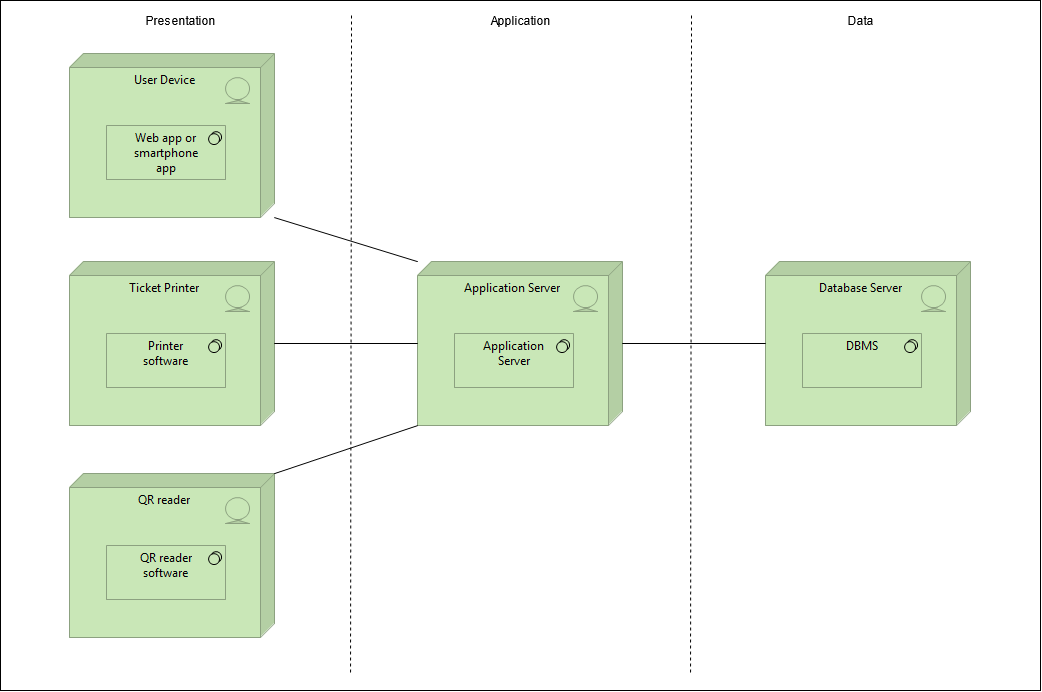
\includegraphics[scale=0.4]{Images/Archimate.png}\\
This image shows the high level representation of the three-layer architecture, where we have all the devices used to interact with the user and their respective software, that have to connect to the application server, which is able to communicate with the database server.\\
Although very simple, this high level view shows how a three tier architecture can provide more flexibility to the system, splitting the server side in two logical layers. It is also very useful from a security viewpoint: in fact the data are kept separated from the user by the application layer, so that all sensitive information are protected from undesired access.
\newpage
Let us now have a more in-depth look at the system architecture.\\
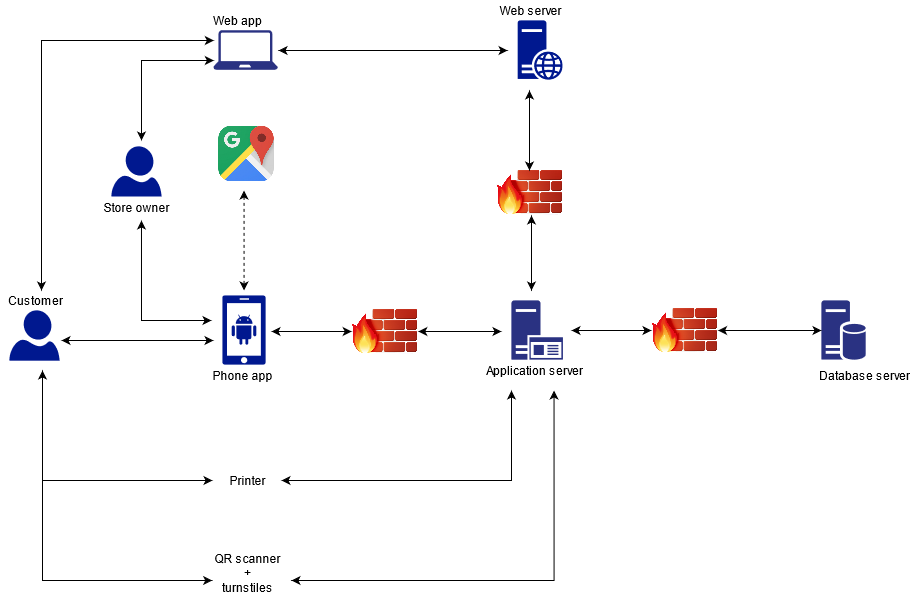
\includegraphics[scale=0.5]{Images/System Architecture.png}\\
Here we can better see how each tier of the previously defined architecture is mapped in the system. The customer is capable to interact with the system in several ways: through the phone app on his smartphone, by the web app on his computer, using the printer outside the store (in order to create an on premise reservation) or via QR scanner, which unlocks the turnstiles and validate enter and exit from the store. In order to provide an estimation of the travel time from the location of the customer to the store, the system uses the GPS technology through the Google Maps API.\\
The store owner, from his/her side, can only access the system from the web app or the phone application; this is because in the role of owner he/she does not need to access the market, and use the system only to control occupation and statistics of the stores.\\
The web app does not communicate directly with the application server, but must traverse the web server, which provide the web pages to the browser.\\
The application server is protected from the outside by a first firewall, which creates a demilitarized zone for it. Then, it communicates with the database server, which contains the database management system, through a second and more restrictive firewall, that isolate the database from possible attacks. This double firewall ensures the security properties for the system.\\
In order to create reservations, the clients must communicate synchronously with the server, as they have no information on the queue. The application server, then communicates synchronously with the database server to retrieve information or asynchronously to store information when needed.\\
In the image above the server element must not be considered as a single machine: if so the architecture would be poorly scalable, and heavy traffic would make the system crash. To guarantee scalability we use a node replication approach, which involves the use of a node balancer which redirect the traffic between multiple servers.\\
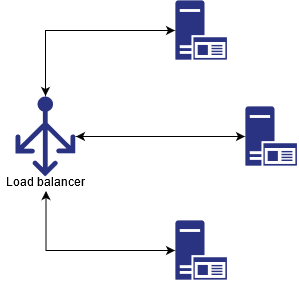
\includegraphics[scale=0.5]{Images/LoadBalancer.png}\\
This image show an example of how this method works for the application tier: in this case the load balancer splits the work between three application servers, but of course there might be more. Moreover this approach is used also for the web server and the database server, according to the needs of the system.\\
Until now we have used an informal view of the architecture; in the next sections we will keep deepening the architecture and its characteristics.\\
\subsection{Component View}
Here we display the main component architecture of our S2B. Since the ApplicationServer contains all the business logic, we will describe in detail the structure of its subcomponents.\\\\
\begin{flushleft}
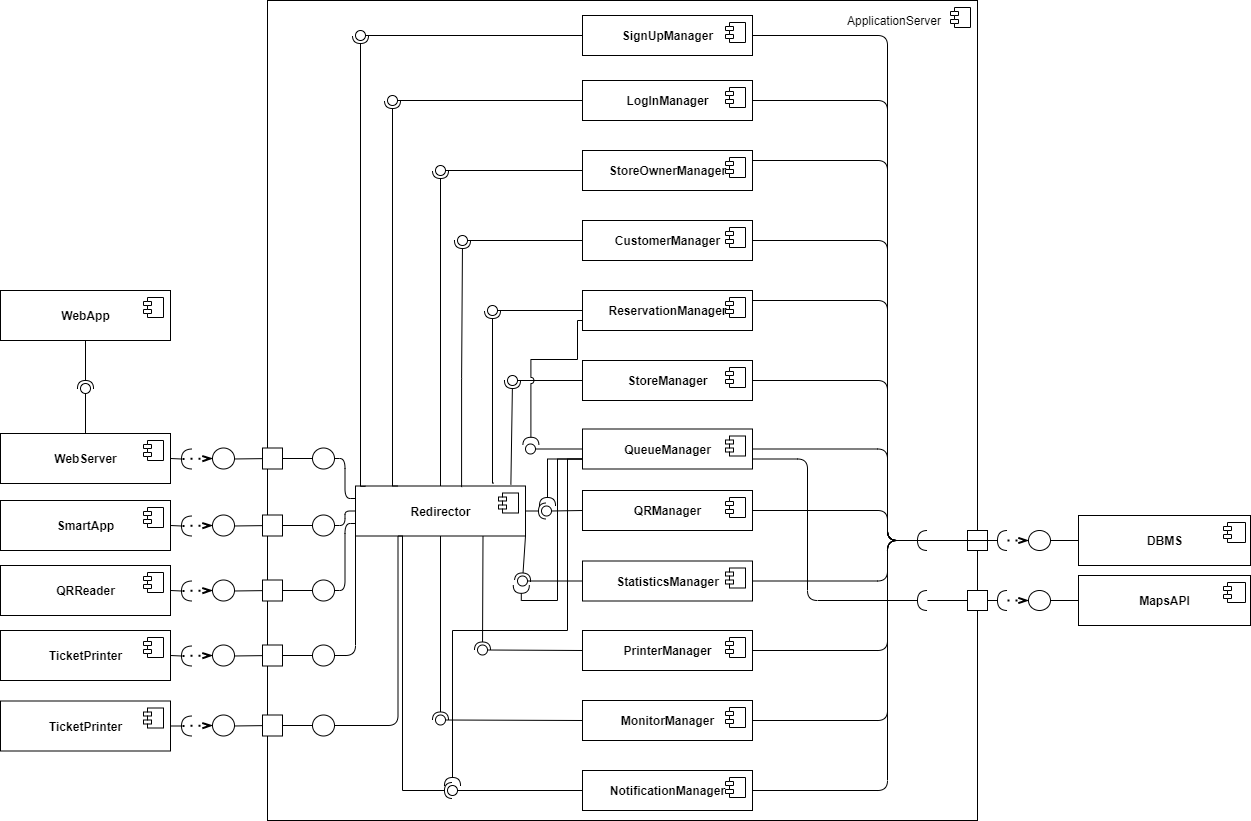
\includegraphics[scale=0.3]{Images/Component.png}
\end{flushleft}
\subsubsection{WebApp}
This component allows customer and store owners to access their respective services on a computer. It requires a WebServer.
\subsubsection{WebServer}
This component communicates directly with the ApplicationServer and serves web pages to implement the WebApp component.
\subsubsection{SmartApp}
This component allows customers and store owners to access their respective services on a smartphone, by interfacing with the ApplicationServer. It is composed of the following subcomponents:
\paragraph{StoreOwnerService}Allows the store owner to access the functionalities that the system reserved to him/her.
\paragraph{CustomerService}Allows the customer to access the functionalities that the system reserved to him/her.
\paragraph{NotificationService}Periodically retrieve the waiting time from the NotificationManager and calls MapsAPI to get the time to reach the store from the current position and if it is greater or equal to the waiting time it notifies the customer.
\subsubsection{QRReader}
This component reads user provided QRCodes and sends them to the ApplicationServer, thus enabling authentication for turnstiles.
\subsubsection{TicketPrinter}
This component accepts a user document and after having validated it through the ApplicationServer, it prints a reservation ticket with a QR.
\subsubsection{StoreMonitor}
This component updates periodically calling the ApplicationServer, which provides it with the number of the last authorized reservation, thus notifying customers in front of the store when they can enter.
\subsubsection{Redirector}
This component provides an external interface for the previously described components, and allows them to communicate with the components that are located within the ApplicationServer, that we describe below.
\subsubsection{AccessManager}
This component allows users to connect to the services, via sign up and login.
\paragraph{SignupManager}
This component allows customers and store owners that provide a valid identification document to register to the service, thus gaining access to its functionalities, provided that they log in. It is called through WebApp or SmartApp, and needs to access the DBMS to search for existing users with same identification document (to avoid duplication), and to create a new user.
\paragraph{LoginManager}
This component allows customers and store owners to log in the service, thus gaining access to its functionalities. It is called by WebApp and SmartApp components, and needs to access the DBMS to verify user credentials against the stored ones.
\subsubsection{UserManager}
This component allows users to change their profile.
\paragraph{StoreOwnerManager}
This component is accessed through WebApp or SmartApp and allows store owners to edit their credentials (obtained during sign up process), thus it needs access to DBMS.
\paragraph{CustomerManager}
This component is accessed through WebApp or SmartApp and allows customers to edit their credentials (obtained during sign up process), thus it needs access to DBMS.
\subsubsection{ReservationManager}
This component is accessed through WebApp or SmartApp by customers and allows them to send a reservation for a specific store, to delete an existing reservation, or to view status of non expired reservations (QR code, position in queue, status) by accessing QueueManager. It needs to access DBMS to retireve the list of the departments of the store that the reservation targets and, in case of an immediate reservation, to verify that the store is open at the current time. It needs access to DBMS also to fetch the list of user reservation along with their information, and to delete them if required. Whenever a customer creates a reservation it is saved into the database.
\subsubsection{StoreManager}
This component is accessed through WebApp or SmartApp, and allows store owners to view owned stores, add new stores, delete existing stores or update information of existing stores, such as the list of departments and their respective maximum occupation. It needs to access the DBMS to execute the previous functions.
\subsubsection{QueueManager}
This component contains the information about the people that are currently waiting to enter the store and those that are already inside it.\\
It is accessed by the ReservationManager to add or remove a reservation from a queue of a specific store.
It is also accessed by the QRManager whenever an authorized customer wants to view the QR and when he/she enters or exits the store.
Finally it is accessed by NotificationManager and MonitorManager respectively in order to get the list of the customers currently waiting and the number of the last authorized customer.\\
It needs access to DBMS to update the status of each reservation and entry and exit times. It checks periodically the number of customers currently present and the maximum occupation for every store and computes an estimated time that customers have to wait before gaining authorization to enter a specific store if such store has already reached maximum occupation.\\
This component accesses StatisticsManager to improve the computation of the time a customer needs to wait before being authorized to enter the store.
\subsubsection{QRManager}
This component accesses QueueManager whenever a customer needs to view a QR for a reservation: if a QR has already been generated for that reservation it is returned to QRManager, otherwise it is generated by QRManager and sent to QueueManager. When QRReader reads a QR code from a customer it calls QRManager, that accesses QueueManager to check that the reservation is existing and authorized, and if so it send the entry/exit time to the QueueManager and returns the QRReader the permission to unlock turnstile.
\subsubsection{StatisticsManager}
This component is accessed by QueueManager to improve the estimate of the time that a customer needs to wait before being authorized to enter a specific store. This component is accessed by a store owner through WebApp or SmartApp to visualize statistics. This component accesses the DBMS periodically to obtain the data with which to generate the statistics, and to save such statistics.
\subsubsection{PrinterManager}
This component allows the store owner with WebApp or SmartApp to register a TicketPrinter. This component also allows customer identification through TicketPrinter by validating a provided identification document. This component needs to access the DBMS to register or unregister instances of TicketPrinter.
\subsubsection{MonitorManager}
This component allows to update periodically a StoreMonitor. It retrieves from the QueueManager the number of the last authorized reservation.
\subsubsection{NotificationManager}
This component is accessed by the NotificationService to retrieve the wait time. This component periodically accesses the QueueManager to get this information.
\subsubsection{MapsAPI}
This component accesses an external mapping service (i.e. GoogleMaps) to compute the estimated time to reach the store from the current position of the device with the selected means of transport.
\subsubsection{DBMS}
This component is the DataBase Management System accessed by the ApplicationServer to perform create/read/update/delete operations on the DB.
\subsubsection{Additional specification}
For what concerns the smartphone application, it is a thick client: in fact beside the presentation logic, it contains a small part of the application logic. Indeed, the phone app can check the validity of the information inserted by the user when creating a reservation and, more importantly, it checks when it is time to notify the customer about its turn to reach the store, based on the position of the device and the position of the store (received by the server). It is important that the phone app does this computations, because the position of the customer, necessary to know how long will it take to go to the market, can only be detected by the end device.\\
The web app, of course, is instead a thin client, because, being it a browser application, will only work on the presentation logic, to show the interface to the user.\\
In order to guarantee the reliability of the system, both the web servers and the application servers must be replicated, so that in case of one of them goes down the application can still work.\\
The load balancer, that in one of the previous diagram has been represented as a single component, may become overloaded by the requests. To prevent this it must be replicated too.
\subsection{Deployment View}
The following image shows the deployment diagram of the system by presenting the distribution (deployment) of software artifacts to the nodes, i.e. the deployment targets.
\begin{flushleft}
	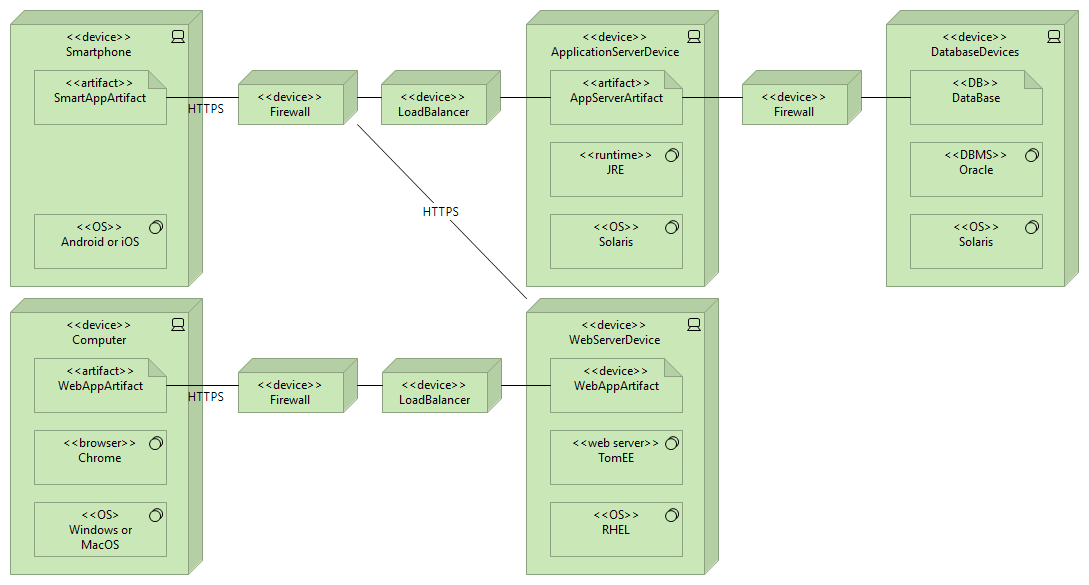
\includegraphics[scale=0.45]{Images/Deployment.png}
\end{flushleft}
Here we describe the components of the deployment view:
\subsubsection{Smartphone}
The customers and the store owners can access the functionalities of the system through a smartphone, that communicates through a firewall and a load balancer with the ApplicationServerDevice.\\
The SmartAppArtifact allows communication between the Smartphone and the ApplicationServerDevice, and its operation is supported by the operative system of the smartphone, either Android or iOS.
\subsubsection{Computer}
The customers and the store owners can access the functionalities of the system through a computer that communicates through a firewall and a load balancer with the WebServerDevice which in turn is connected through a firewall and a load balancer with an ApplicationServerDevice.\\
The WebAppArtifact will be downloaded from the WebServerDevice and it will be shown by the browser installed on the device which we assume for simplicity to be Chrome, whose operation is supported by the operating system of the Computer, either Windows or MacOs. 
\subsubsection{Firewall}
The firewalls allow to separate the different parts of the system: the DatabaseDevice is isolated from the ApplicationServerDevice, which in turn is isolated from the Smartphone and the WebServerdevice, which in turn is isolated from the Computer.
\subsubsection{LoadBalancer}
The LoadBalancer allow to balance the load of the system on the replicated ApplicationServerDevices and WebServerDevices.
\subsubsection{ApplicationServerDevice}
This device implements the main business logic of our system. It is accessed by Smartphone and Computer devices to make use of the functionalities offered by the system. It is supported by a DatabaseDevice that allows the ApplicationDevice to create, read, update and delete all the information necessary for the correct functioning of the system.\\
The AppServerArtifact is run by the JRE which in turn is supported by the Solaris operating system.
\subsubsection{WebServerDevice}
This device allows customers and store owners to access their respective services by using Java RMI to communicate with the ApplicationServerDevice.\\
The web server TomEE will server the browser the artifact it needs to show to the users. This web server's operation will be supported by Red Hat Linux Enterprise operating system.
\subsubsection{DatabaseDevice}
This device allows the ApplicationServerDevice to create, read, update, delete information that supports the system operation.\\
The DataBase is managed by the Oracle DBMS which in turn is supported by Oracle Solaris.

%------------------------------------------------------------------------------------------------------------------------------------------------
\clearpage
{\color{Blue}{\section{User Interface Design}}}
\label{sect:requirements}
In the Requirements And Specification Document, Section 3.1.1  User interfaces, we already provide many mockups of the user interface for the smartphone app. Here we present an additional one to exemplify the interface of the web app for the creation of an immediate reservation.\\
\begin{figure}[H]
	\noindent
	\makebox[\textwidth]{ 
		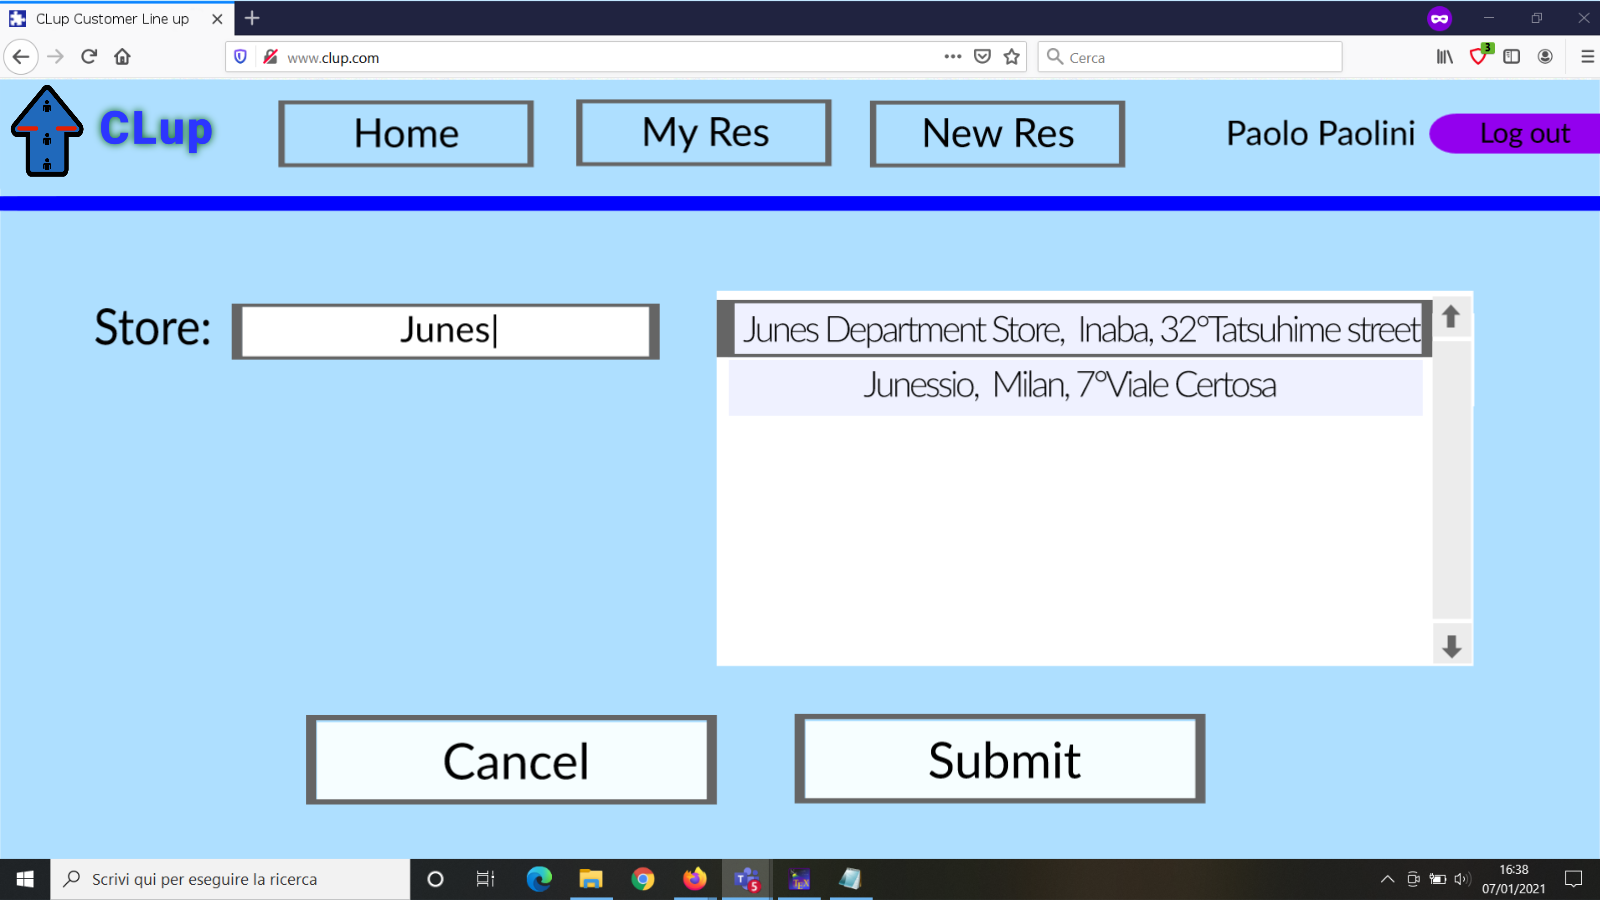
\includegraphics[scale=0.3]{Images/WebAppMockUp.png}}
	\caption{WebApp mockup}
\end{figure}

%------------------------------------------------------------------------------------------------------------------------------------------------
\clearpage
{\color{Blue}{\section{Requirements Traceability}}}
\label{sect:alloy}
\subsection{External interface requirements}
\subsubsection{User interfaces}
There are two categories of users that have different interface requirements:
\begin{itemize}
	\item {\bfseries Customers}\\
	Customers belong to all demographics so a user friendly interface is needed. The customer is presented with a main menu which allows him/her to:
	\begin{itemize}
		\item line up immediately (immediate reservation) at a specific store
		\item book a visit (future reservation) at a specific store
		\item view and delete existing reservations
	\end{itemize}
	The customer will receive a notification when it is time for him/her to depart to reach the shop.\\\\
	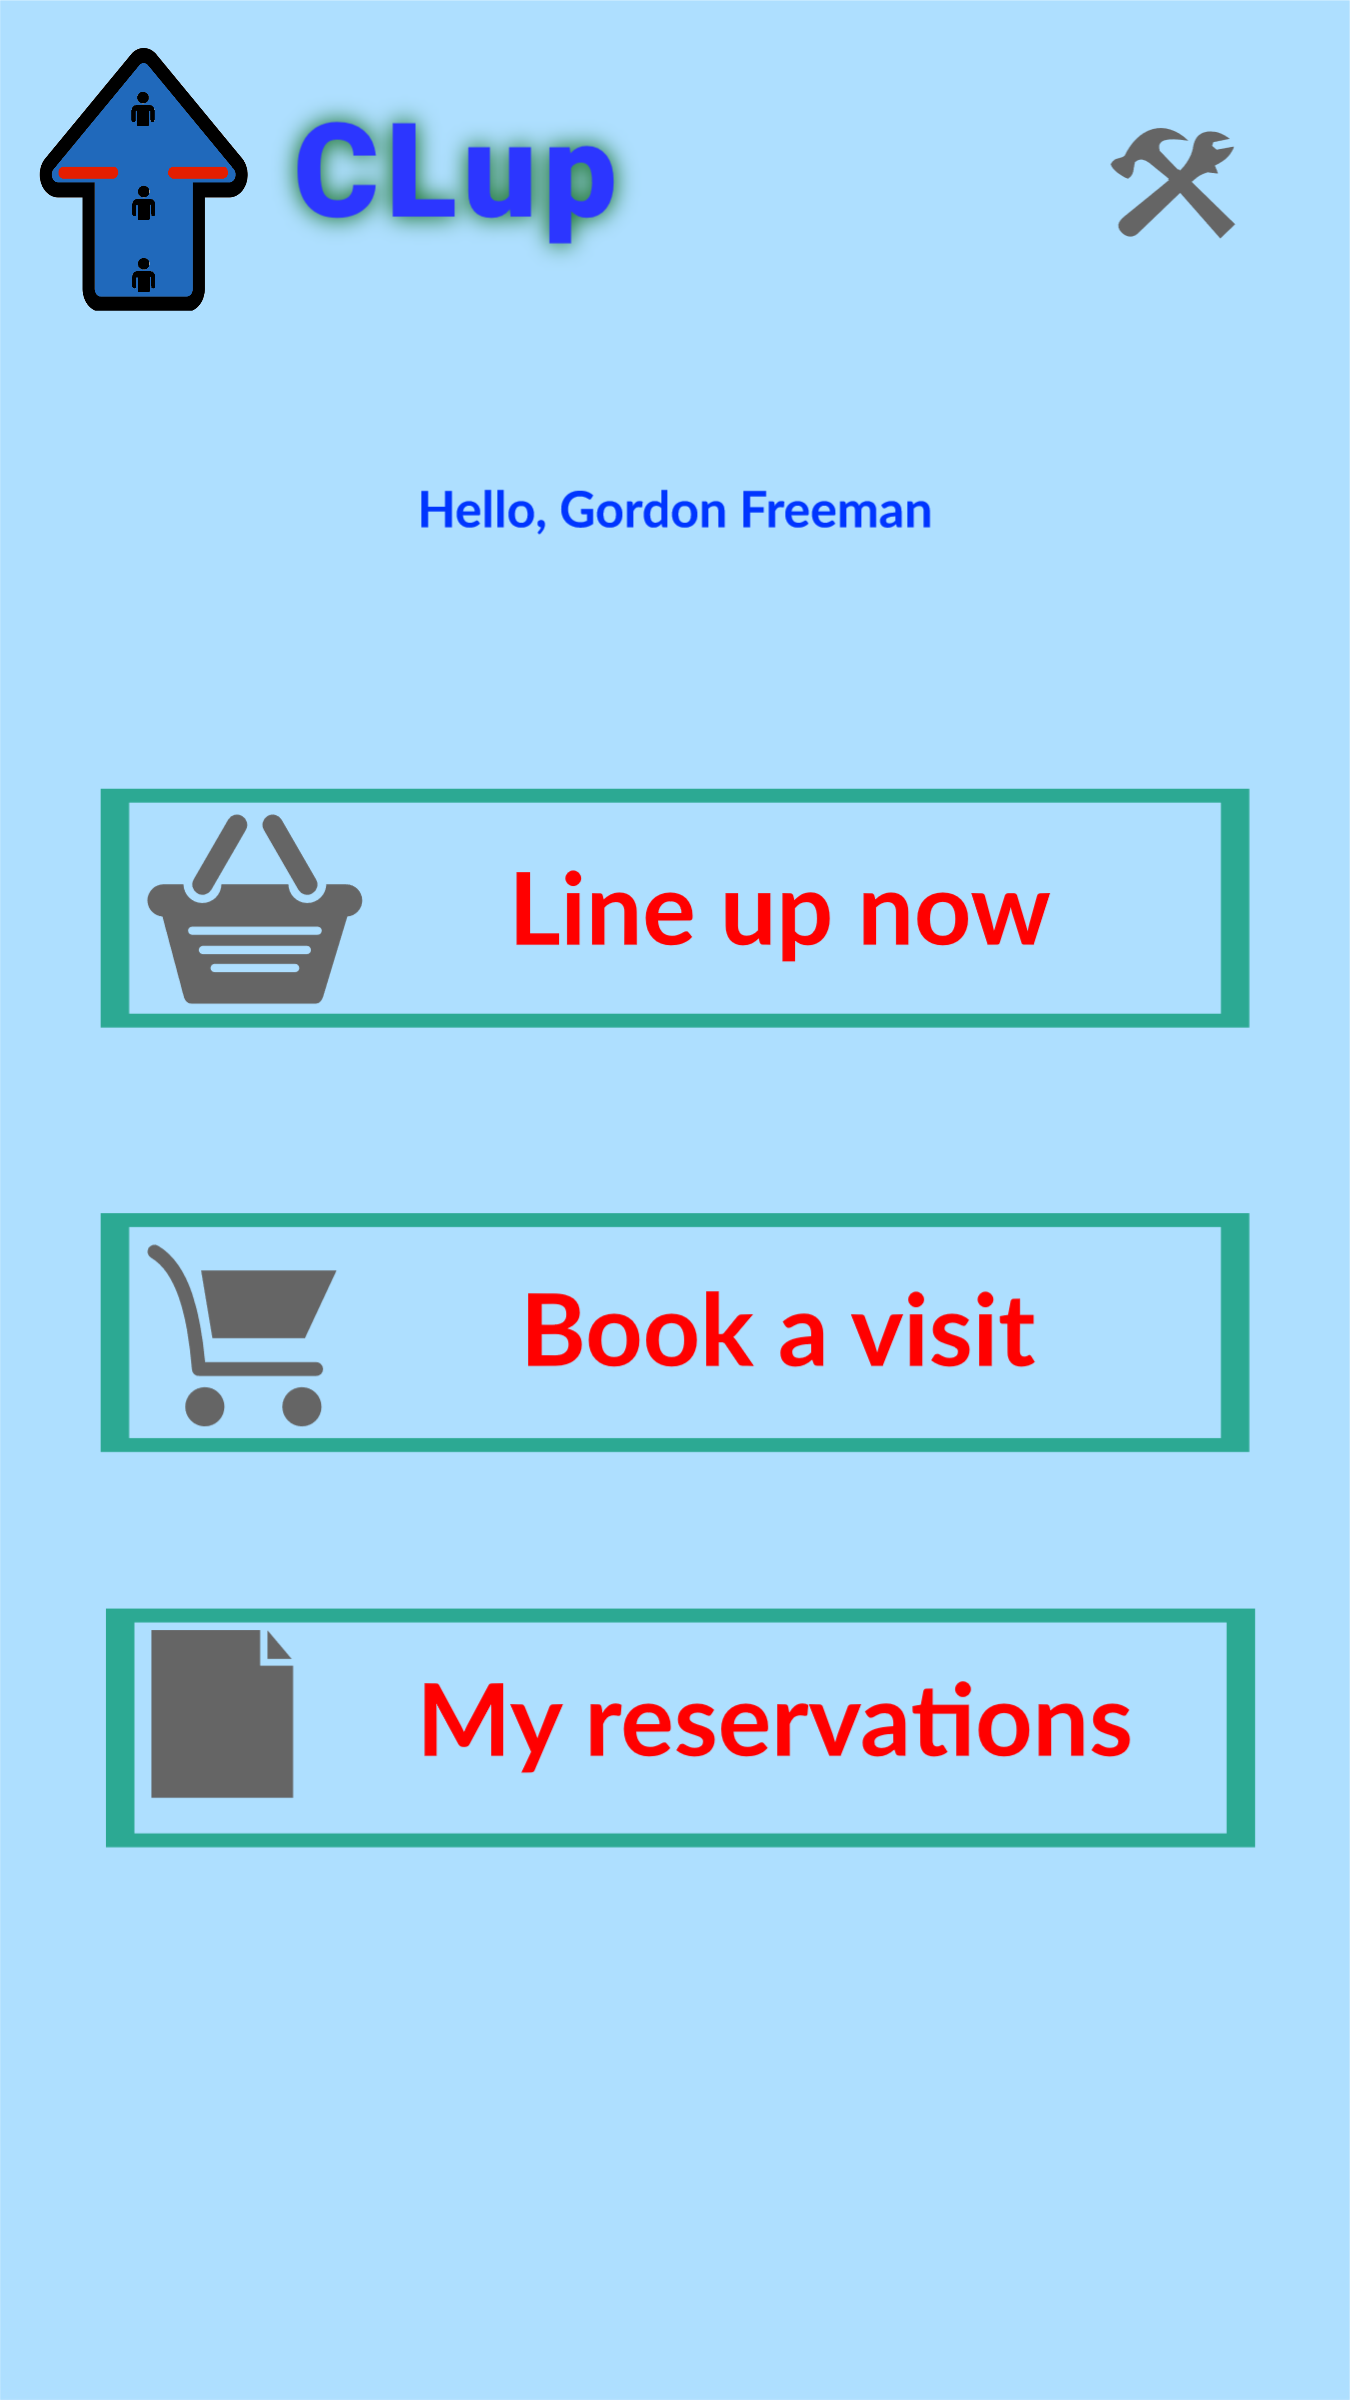
\includegraphics[scale=0.1]{Images/MainMenuCustomer.png}
	\qquad
	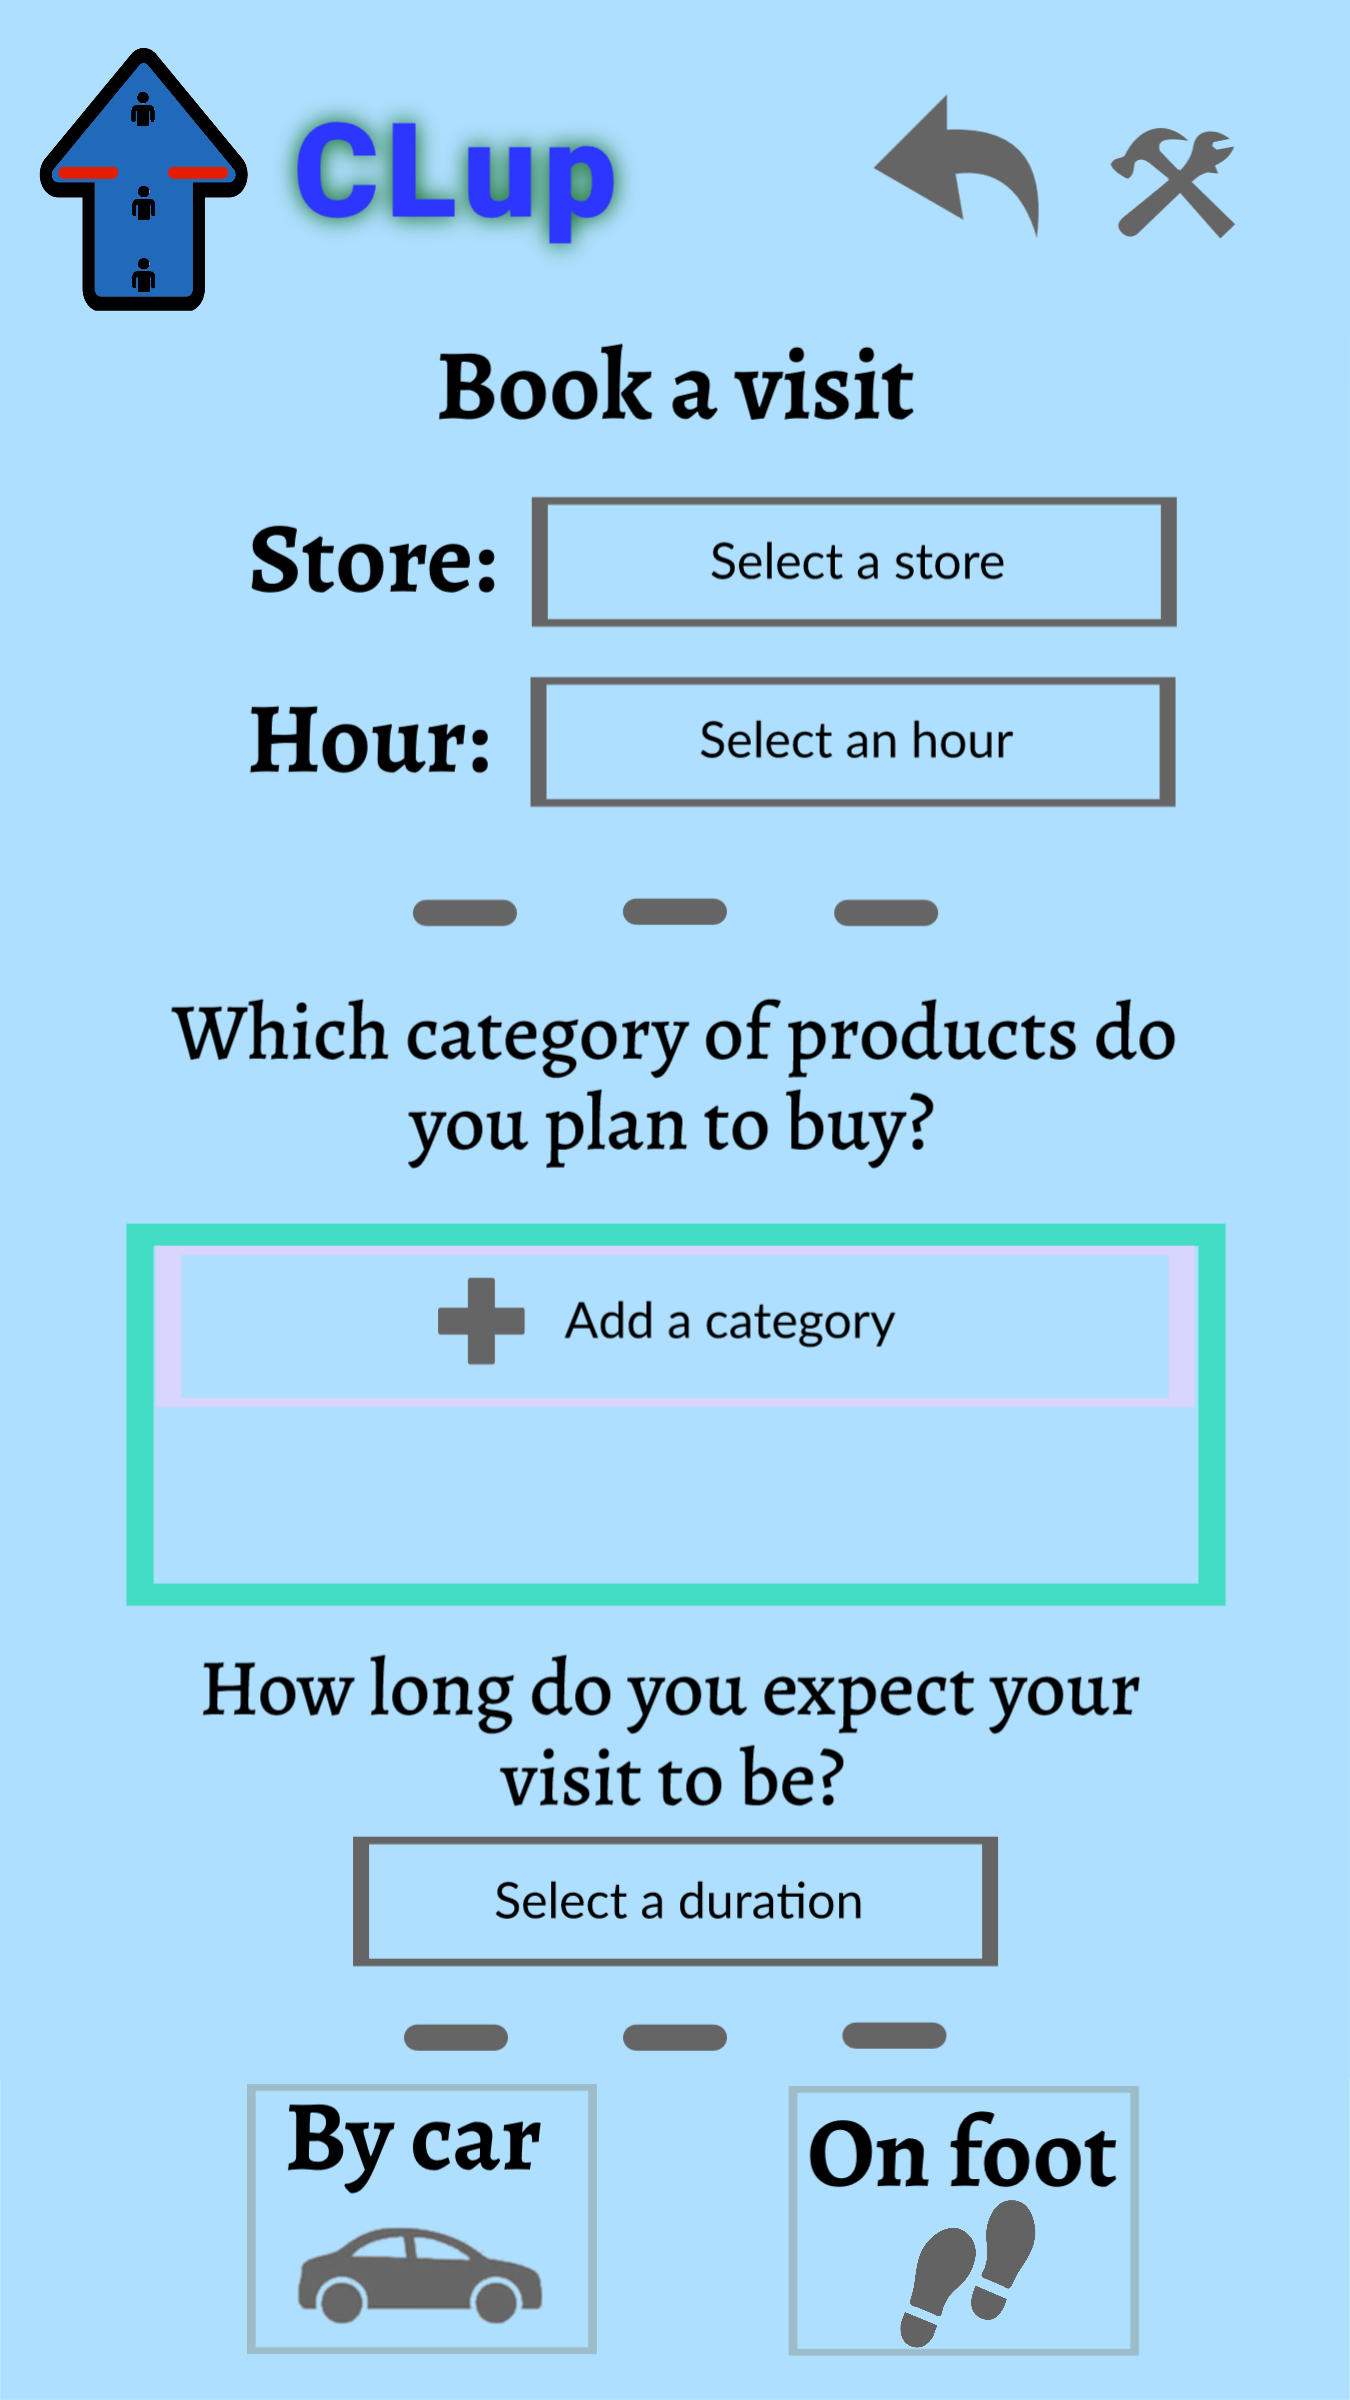
\includegraphics[scale=0.1]{Images/BookAVisit.png}
	\qquad
	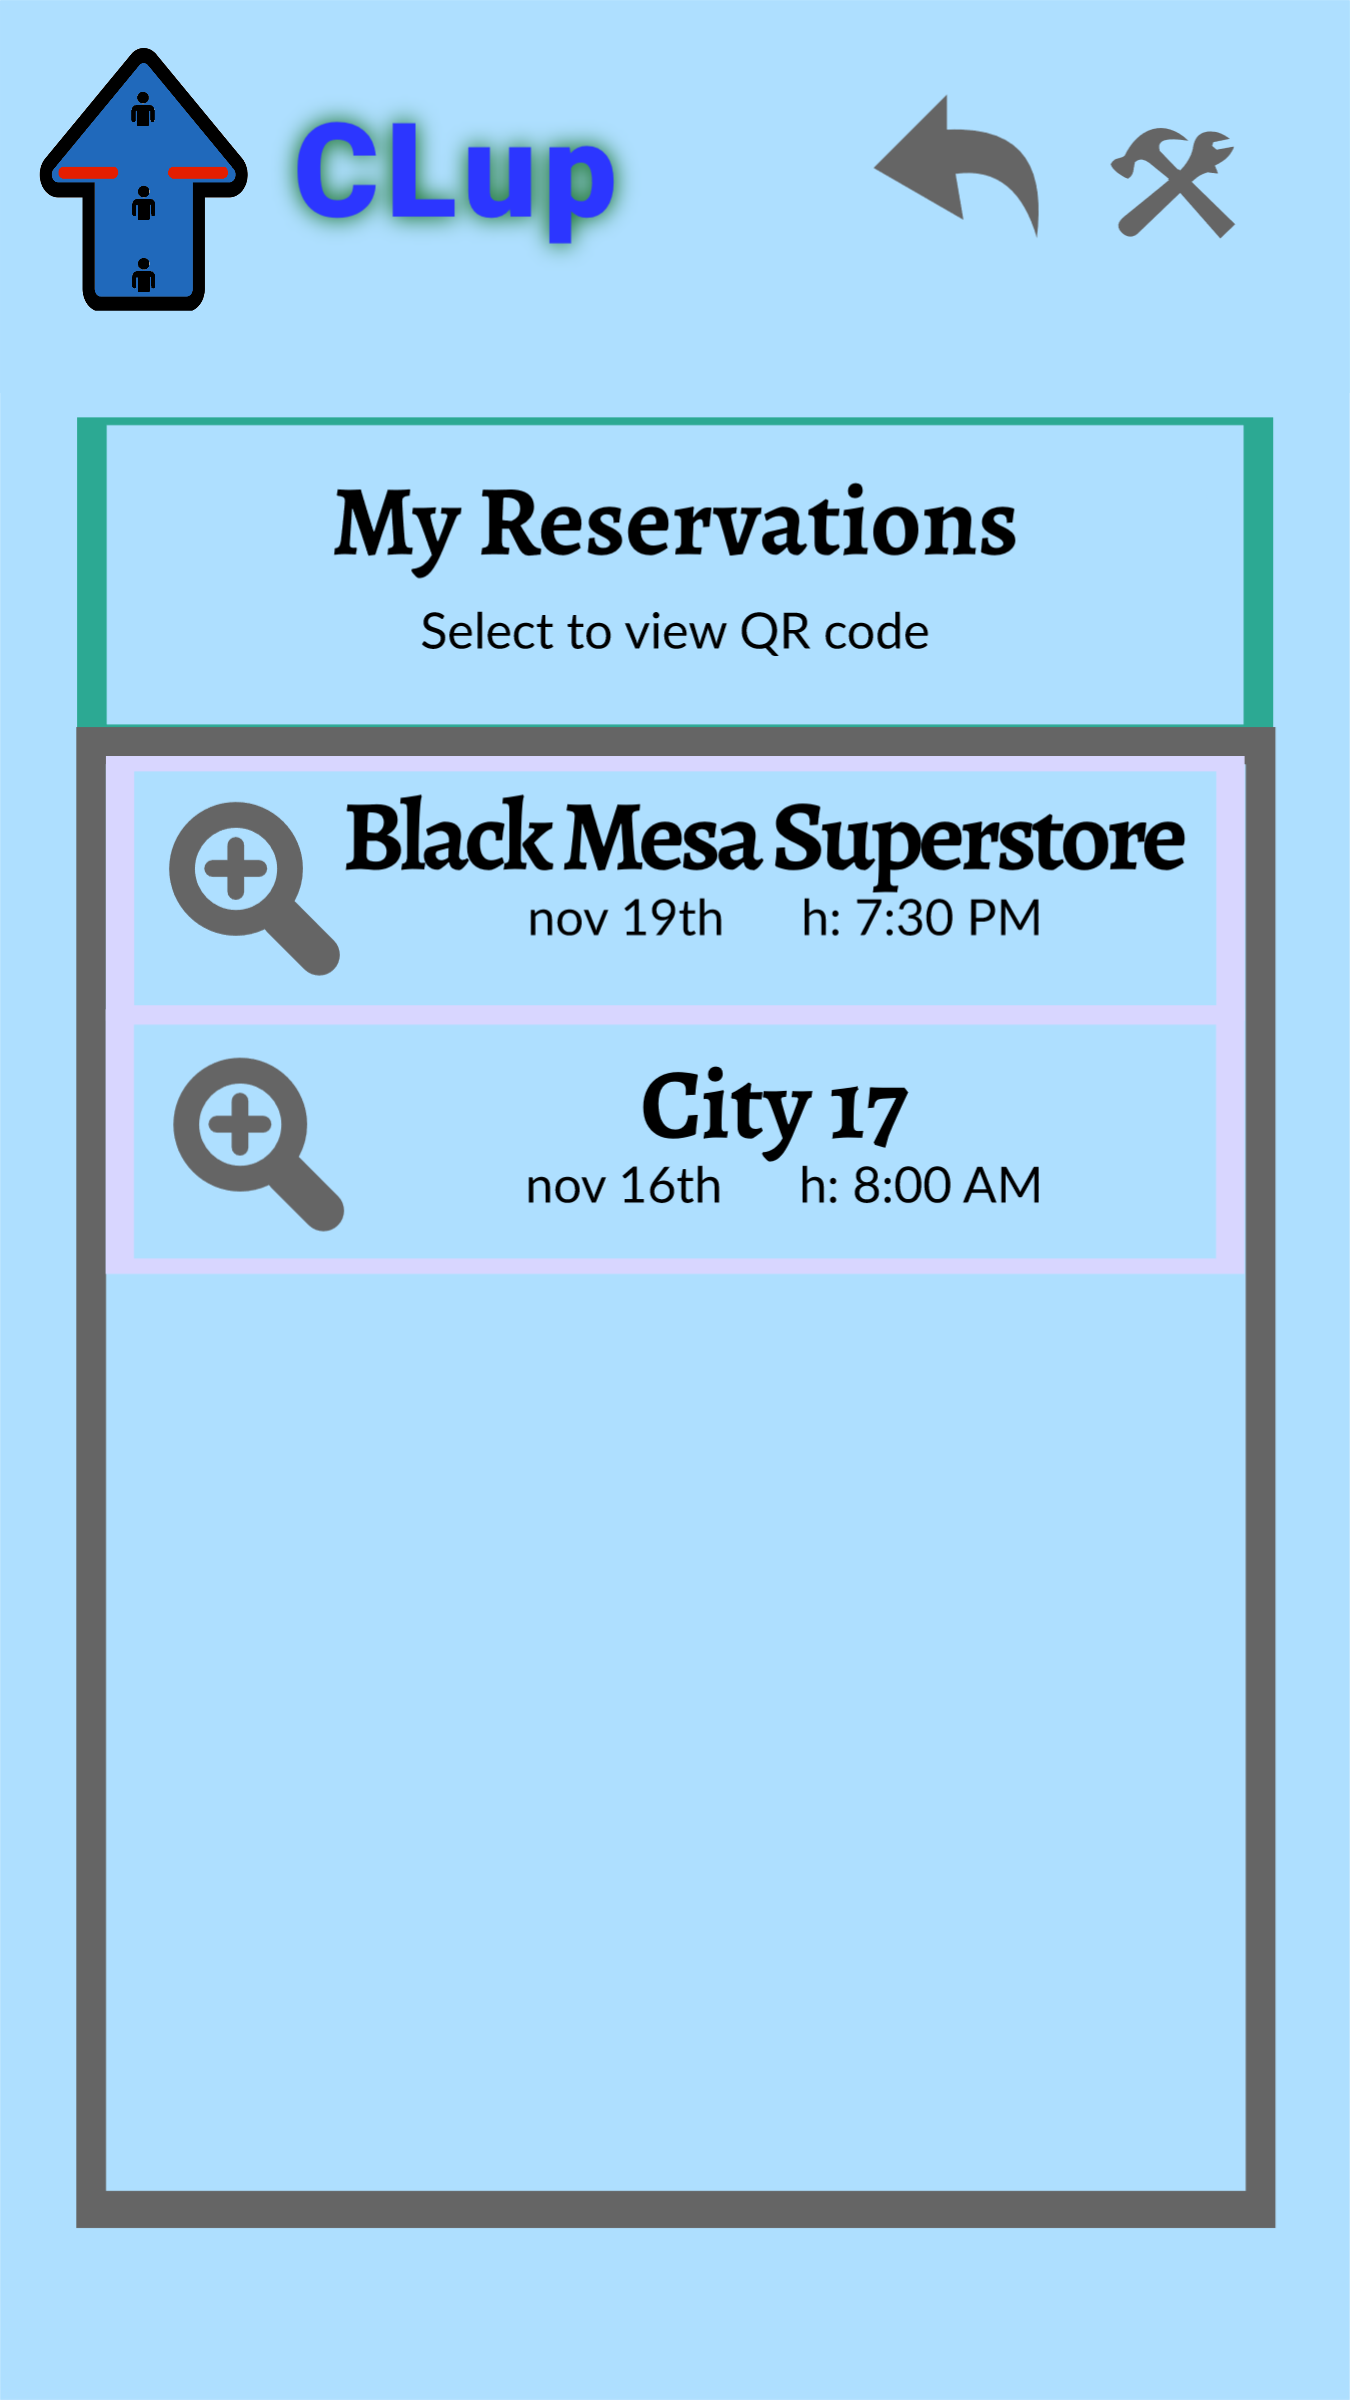
\includegraphics[scale=0.1]{Images/ShowReservations.png}
	\item {\bfseries Store owners}\\
	The store owner is presented with a main menu from which he/she can:
		\begin{itemize}
		\item register a store to the system
		\item delete a store from the system
		\item view and edit occupation for currently registered stores
	\end{itemize}
	\begin{figure}[!htb]
		\centering
		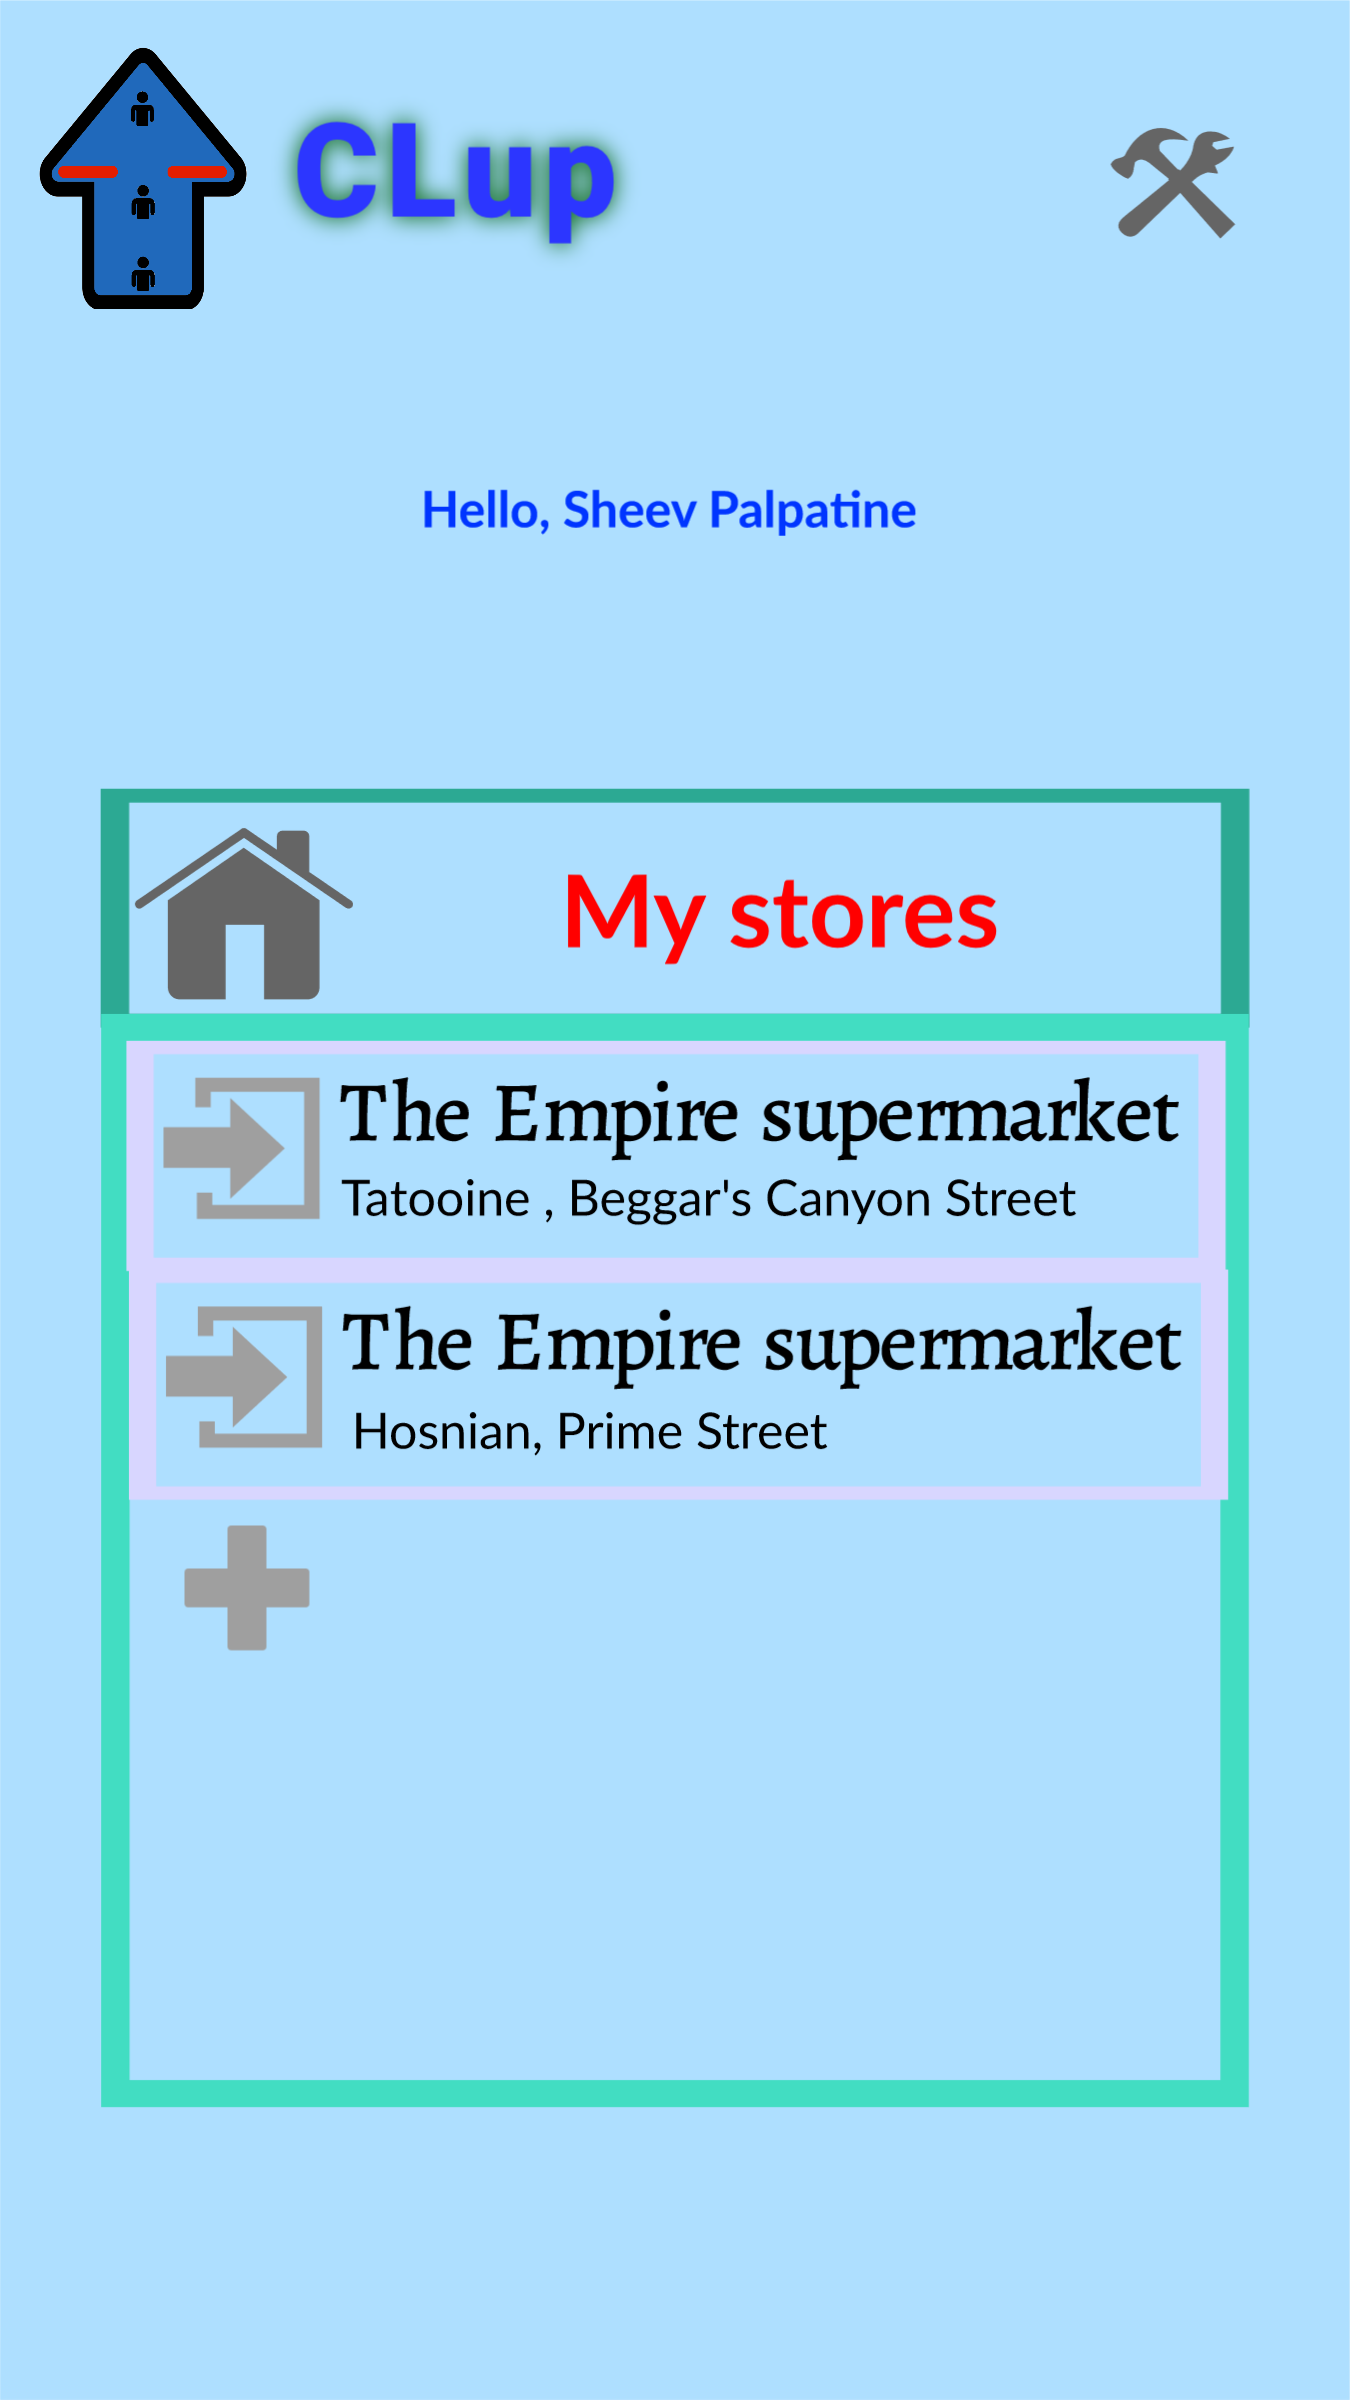
\includegraphics[scale=0.1]{Images/MainMenuOwner.png}
		\qquad \qquad
		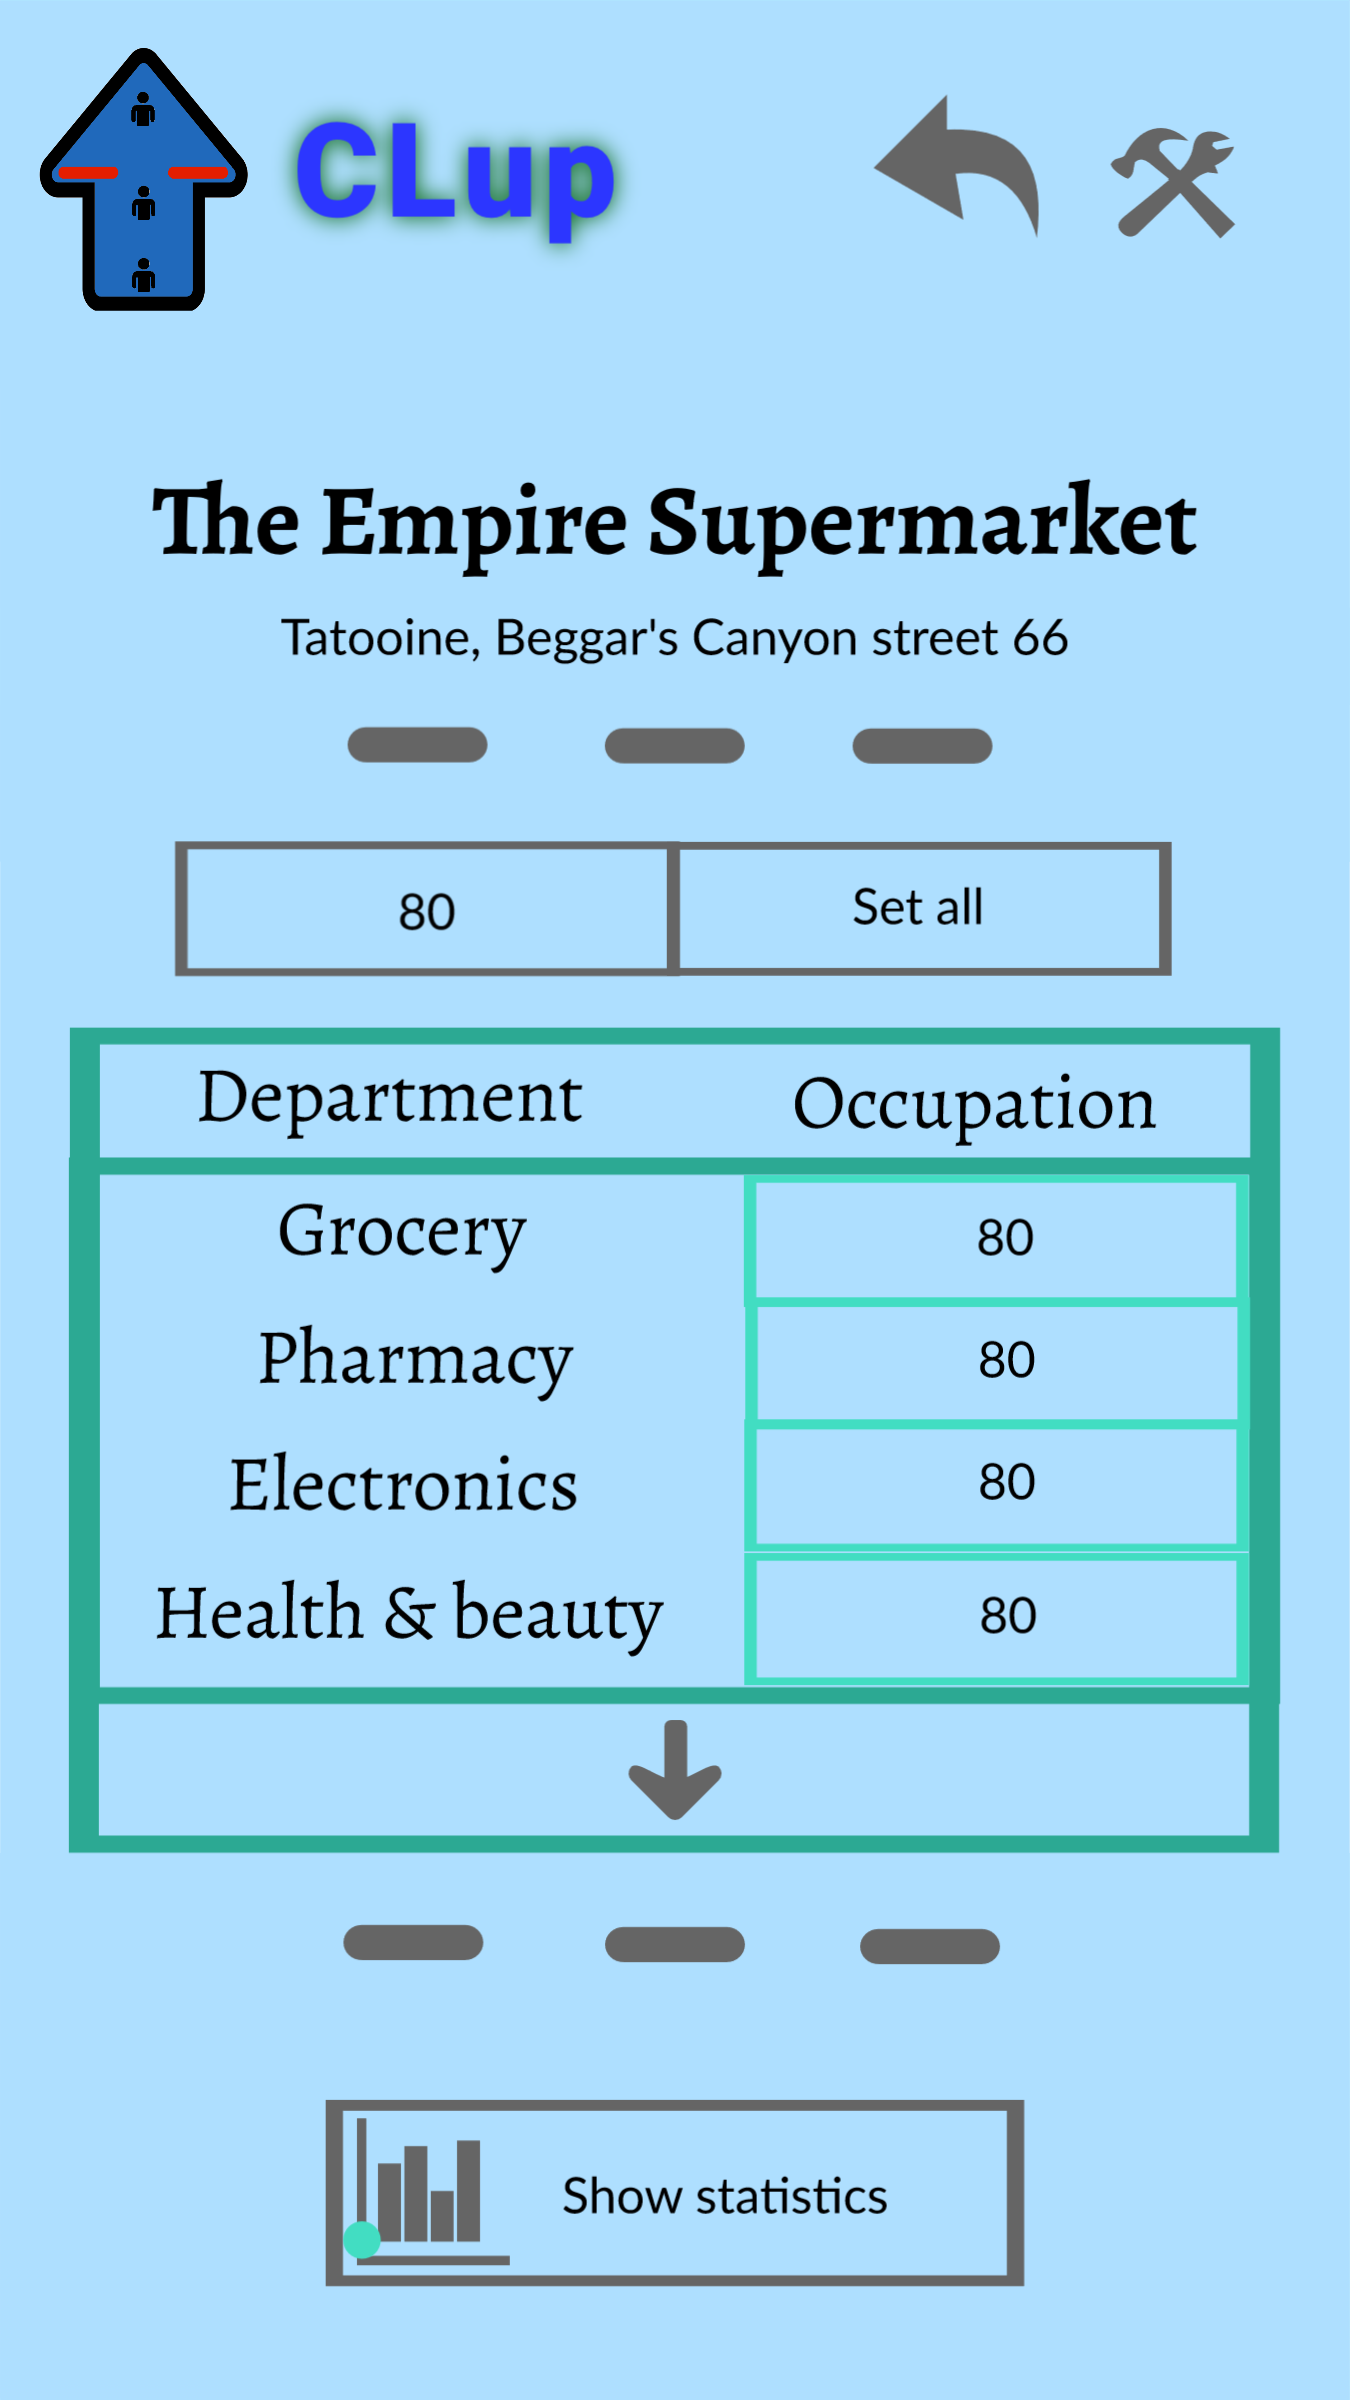
\includegraphics[scale=0.1]{Images/ModifyOccupation.png}
	\end{figure}
	\newpage
\end{itemize}
\subsubsection{Hardware interfaces}
The S2B requires the following hardware interfaces:
\begin{enumerate}
	\item {\bfseries Computer or smartphone}\\
	Users will need a computer or a smartphone to access the system's services which are provided via an application (only for smartphone owners) and a web application. Only users with an application will be able to receive notifications that alert them when it is time for them to depart and reach the store.
	\item {\bfseries Turnstiles}\\
	Turnstiles allow authorized customers to enter or exit the store by providing a means of identification. (i.e. QR, NFC)
	\item {\bfseries Ticket printer}\\
	The ticket printers located outside stores allows potential customers to queue up on premise provided that they identify themselves (e.g. social security card).
	\item \textbf{Monitor}\\
	A monitor located outside stores allows customers that queue up on premise to know when it is time for them to access the store.
\end{enumerate}

\subsubsection{Software interfaces}
The system uses a public API to locate the customer and provide him/her with notifications about the time he will need to depart to reach the store.

\subsubsection{Communication interfaces}
Customers can access the system through a working internet connection.

\subsection{Functional requirements}
\subsubsection{List of requirements}
\begin{enumerate}[label=R\arabic*]
	\item Turnstiles unlock if and only if activated by authorized customers.
	\item The number of customers in each department of the store never exceeds the occupation set by the owner.
	\item The monitor outside the store displays the number of the last authorized customer.
	\item The system allows customers and store owners to register and log in.
	\item The system validates the authenticity of the identifying information provided.
	\item The system allows customers to search for a store among those registered by their owners.
	\item Registered customers can send a reservation request to the system.
	\item Non registered customers with an identifying document can request reservations through the printer.
	\item Registered customers that book a visit can specify estimated visit duration.
	\item Registered customers that book a visit can specify desired product categories.
	\item The system provides customers with a QR code to enter the store once authorized.
	\item The system uses gathered data to build statistics.
	\item Registered customers with a smartphone are alerted when their turn is near.

	\item Registered customers can delete a pending or authorized reservation.
	\item Authorized reservations expire if they do not become current in a certain time window (specified by store owner)
	\item Registered customers must specify desired means of transport while requesting a reservation.
	\item Reservations are authorized according to a FIFO policy
\end{enumerate}
\subsubsection{Mapping on requirements}
\begin{tabular}{ | m{3cm} | m{5cm} | m{9cm} | }
	\hline
	G1 & D1, D2, D5, D6, D8, D9 & R1, R2, R4, R5, R6, R7, R11, R16, R17\\
	\hline
	G2 & D1, D2, D3, D4, D5, D6 & R1, R2, R3, R5, R8, R11, R17\\
	\hline
	G3 & D1, D2, D3, D4, D5, D6, D8, D9 & R1, R2, R3, R4, R5, R6, R7, R9, R10, R11, R16, R17\\
	\hline
	G4 & D1, D2, D5, D8, D9 & R1, R2 \\
	\hline
	G5 & D8, D9 & R9, R12, R14, R15\\
	\hline
	G6 & D4, D7, D8, D9 & R3, R13\\
	\hline
\end{tabular}
\newpage
Here we remind the goals for ease of use:
\begin{enumerate}[label=G\arabic*]
	\item CLup should allow customers to queue up remotely
	\item CLup should allow customers to queue up on premise
	\item CLup should allow customers to book future visits to stores
	\item CLup should allow store owners to regulate the maximum number of customers in their stores
	\item CLup should provide the customer with a reasonably precise estimate of waiting time
	\item CLup should alert the customers when it is time to get to the shop taking into account travel time
\end{enumerate}

Here we remind the domain assumptions for ease of use:
\begin{enumerate}[label=D\arabic*]
	\item The stores have QR activated turnstiles.
	\item Turnstiles let one and only one person in each time they unlock.
	\item Outside stores is a social security card activated ticket printer.
	\item Outside stores there is a monitor.
	\item There is no way for a customer to enter a store except from entrance and exit.
	\item Each customer has either a telephone number or an identification document.
	\item When provided, user location has maximum error of 5 meters.
	\item To register to the S2B users must have either a smartphone or a computer.
	\item To register and use the S2B users must have an internet connection.
\end{enumerate}
\subsubsection{Use case diagram}
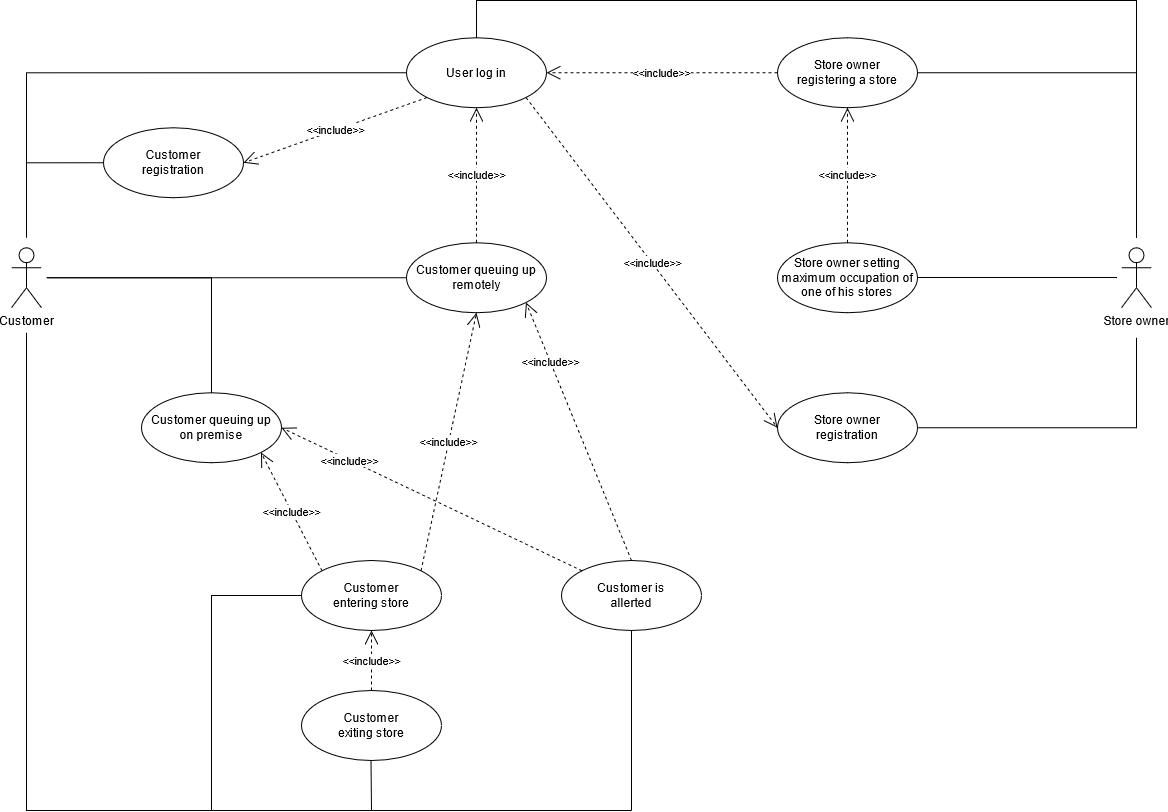
\includegraphics[scale=0.4]{Images/Use Case Diagram.png}
\newpage
\subsubsection{Use cases}
\paragraph{Customer registration}
\begin{flushleft}
	\begin{tabular} { | m{3cm} | m{10cm} | }
		\hline
		Name & Customer registration\\
		\hline
		Actors & Customer\\
		\hline
		Entry condition & Customer has opened the smartphone application or the web app on his computer but has not logged in\\
		\hline
		Event flow & \begin{enumerate}
			\item a registration menu is provided to the customer
			\item from such menu the customer selects the option to sign up as customer
			\item the customer is then prompted to insert identifying information
			\item the customer inserts requested information
			\item the system validates provided information
			\item the system confirms the registration of the customer and saves information provided
		\end{enumerate}\\
		\hline
		Exit conditions & Customer has registered to the system\\
		\hline
		Exceptions & \begin{enumerate}
			\item a customer with same identifying information already exists
			\item validation of identifying information is not successful
			\item the customer decides to cancel the registration
		\end{enumerate}
		If one of the first two events described above occur, the application will alert the customer and provide him with the possibility to retry or go back to the initial menu.\newline If event 3 occurs the customer is redirected to the main page.\\
		\hline
	\end{tabular}
\end{flushleft}
\newpage
\paragraph{Store owner registration}
\begin{flushleft}
	\begin{tabular} { | m{3cm} | m{10cm} | }
		\hline
		Name & Store owner registration\\
		\hline
		Actors & Store owner\\
		\hline
		Entry condition & Store owner has opened the smartphone application or the web app on his computer but has not logged in\\
		\hline
		Event flow & \begin{enumerate}
			\item a registration menu is provided to the store owner
			\item from such menu the store owner selects the option to sign up as store owner
			\item the store owner is then prompted to insert identifying information
			\item the store owner inserts requested information
			\item the system validates provided information
			\item the system confirms the registration of the store owner and saves information provided
		\end{enumerate}\\
		\hline
		Exit conditions & Store owner has registered to the system\\
		\hline
		Exceptions & \begin{enumerate}
			\item a store owner with same identifying information already exists
			\item validation of identifying information is not successful
			\item the store owner decides to cancel the registration
		\end{enumerate}
		If one of the first two events described above occur, the application will alert the store owner and provide him with the possibility to retry or go back to the initial menu.\newline If event 3 occurs the store owner is redirected to the main page.\\
		\hline
	\end{tabular}
\end{flushleft}

\paragraph{User logs in}
\begin{flushleft}
	\begin{tabular} { | m{3cm} | m{10cm} | }
		\hline
		Name & User logs in\\
		\hline
		Actors & Customer or store owner\\
		\hline
		Entry condition & The user has opened the application on his device, and has already registered to the system\\
		\hline
		Event flow & \begin{enumerate}
            \item User chooses to log in from the welcome menu
            \item User identifies him/herself with created credentials
		\end{enumerate}\\
		\hline
		Exit conditions & User is logged in\\
		\hline
		Exceptions & \begin{enumerate}
			\item User credentials are invalid
		\end{enumerate}
		If the event described above occurs, the application will alert the user and allows him to retry\\
		\hline
	\end{tabular}
\end{flushleft}
\newpage
\paragraph{Customer queuing up remotely}
\begin{flushleft}
	\begin{tabular} { | m{3cm} | m{10cm} | }
		\hline
		Name & Customer queuing up remotely\\
		\hline
		Actors & Customer\\
		\hline
		Entry condition & Customer has logged in on the smartphone application or the web app on his computer\\
		\hline
		Event flow & \begin{enumerate}
			\item customer selects to queue up from main menu
			\begin{itemize}
				\item with an immediate reservation
				\item with a future reservation (and optionally inserts desired categories of item he/she intends to buy and how much time he/she intends to spend at the store)
			\end{itemize}
			\item customer selects a store from the list of stores registered to the system
			\item customer specify  whether he is going to reach the store by car or on foot
			\item customer submits reservation request
		\end{enumerate}\\
		\hline
		Exit conditions & Customer reservation is confirmed\\
		\hline
		Exceptions & \begin{enumerate}
			\item customer decides to cancel the reservation
			\item customer requests immediate reservaiton but store is closed at that time
		\end{enumerate}
		If one of the events described above occur, the application will alert the customer and go back to the initial menu\\
		\hline
	\end{tabular}
\end{flushleft}
\newpage
\paragraph{Customer queuing up on premise}
\begin{flushleft}
	\begin{tabular} { | m{3cm} | m{10cm} | }
		\hline
		Name & Customer queuing on premise\\
		\hline
		Actors & Customer\\
		\hline
		Entry condition & Customer has reached the store ticket printer\\
		\hline
		Event flow & \begin{enumerate}
			\item customer selects the option to queue up from main menu of the ticket printer
			\item customer provides the ticket printer with a means of identification (e.g. social security card)
		\end{enumerate}\\
		\hline
		Exit conditions & Customer reservation is confirmed and a ticket is printed containing the following information:
		\begin{itemize}
			\item how much time he needs to wait before being able to enter the store
			\item a progressive number that will allow him to know when his/her turn is
		\end{itemize}\\
		\hline
		Exceptions & \begin{enumerate}
			\item customer decides to cancel the reservation
		\end{enumerate}
		If one of the events described above occur, the application will alert the customer and go back to the initial menu\\
		\hline
	\end{tabular}
\end{flushleft}

\paragraph{Customer entering store}
\begin{flushleft}
	\begin{tabular} { | m{3cm} | m{10cm} | }
		\hline
		Name & Customer entering store\\
		\hline
		Actors & Customer\\
		\hline
		Entry condition & Customer has logged in on the smartphone application and is at the entrance of a store or has printed authorization from the web app\\
		\hline
		Event flow &
		If the customer has not printed the reservation ticket he must use his smartphone:
		\begin{enumerate}
			\item customer selects the option to show existing reservations from main menu of the phone app 
			\item customer selects an existing reservation and if authorized (i.e. it is his turn to enter the store) he/she is given the means to identify him/herself (e.g. display QR or activate NFC)
		\end{enumerate}
		Then the customer identifies him/herself at the turnstiles\\
		\hline
		Exit conditions & Customer enters the store\\
		\hline
		Exceptions & \begin{enumerate}
			\item customer is not authorized to enter the store
		\end{enumerate}
		If the event described above occurs, the turnstiles will not let the customer in\\
		\hline
	\end{tabular}
\end{flushleft}
\newpage
\paragraph{Customer exiting store}
\begin{flushleft}
	\begin{tabular} { | m{3cm} | m{10cm} | }
		\hline
		Name & Customer exiting store\\
		\hline
		Actors & Customer\\
		\hline
		Entry condition & Customer has logged in on the smartphone application and is in a store\\
		\hline
		Event flow &
		If the customer has not printed the reservation ticket he must use his smartphone:
		\begin{enumerate}
			\item customer selects the option to show existing reservations from main menu
			\item customer selects an existing reservation and if authorized (i.e. it is his turn to enter the store) he/she is given the means to identify him/herself (e.g. display QR or activate NFC)
		\end{enumerate}
	    Customer identifies him/herself at the turnstiles\\
		\hline
		Exit conditions & Customer exits the store\\
		\hline
		Exceptions & \\
		\hline
	\end{tabular}
\end{flushleft}

\paragraph{Store owner registering a store}
\begin{flushleft}
	\begin{tabular} { | m{3cm} | m{10cm} | }
		\hline
		Name & Store owner registering a store\\
		\hline
		Actors & Store owner\\
		\hline
		Entry condition & Store owner has logged in on the smartphone application or the web app on his computer\\
		\hline
		Event flow & \begin{enumerate}
			\item store owner selects the option register a store from main menu
			\item store owner inserts necessary information and sets up equipment (i.e. connect printer, monitor and turnstiles to the system)
			\item store owner submits store registration request
		\end{enumerate}\\
		\hline
		Exit conditions & Store registration is confirmed\\
		\hline
		Exceptions & \begin{enumerate}
			\item information is missing or incorrect
			\item equipment is not working properly			\item store owner decides to cancel the store registration
		\end{enumerate}
		If one of the events described above occur, the application will alert the store owner and provide him with the possibility to retry or go back to the initial menu\\
		\hline
	\end{tabular}
\end{flushleft}
\newpage
\paragraph{Store owner setting maximum occupation of a store or a department}
\begin{flushleft}
	\begin{tabular} { | m{3cm} | m{10cm} | }
		\hline
		Name & Store owner setting maximum occupation of a store or a department\\
		\hline
		Actors & Store owner\\
		\hline
		Entry condition & Store owner has logged in on the smartphone application or the web app on his computer\\
		\hline
		Event flow & \begin{enumerate}
			\item store owner selects one of his stores from the list reachable form the main menu
			\item store owner views current occupation of each department of his store, and current occupation threshold
			\item sets the new desired occupation threshold for a department or for the whole store
		\end{enumerate}\\
		\hline
		Exit conditions & The new occupation threshold is set\\
		\hline
		Exceptions & \begin{enumerate}
			\item the threshold value is inadequate
		\end{enumerate}
		If the event described above occurs, the application will alert the store owner and provide him with the possibility to retry or go back to the initial menu\\
		\hline
	\end{tabular}
\end{flushleft}
\paragraph{Customer is alerted}
\begin{flushleft}
	\begin{tabular} { | m{3cm} | m{10cm} | }
		\hline
		Name & Customer is alerted\\
		\hline
		Actors & Customer\\
		\hline
		Entry condition & Customer is logged into his smartphone application and the time he/she needs to wait becomes less or equal to the time he/she needs to reach the store\\
		\hline
		Event flow & \begin{enumerate}
			\item The system sends a notification to the smartphone of the customer
		\end{enumerate}\\
		\hline
		Exit conditions & Customer is notified\\
		\hline
		Exceptions & \begin{enumerate}
			\item the threshold value is inadequate
		\end{enumerate}
		If the event described above occurs, the application will alert the store owner and provide him with the possibility to retry or go back to the initial menu\\
		\hline
	\end{tabular}
\end{flushleft}
\newpage
\subsubsection{Sequence diagrams}
\paragraph{Customer registration}
\begin{flushleft}
	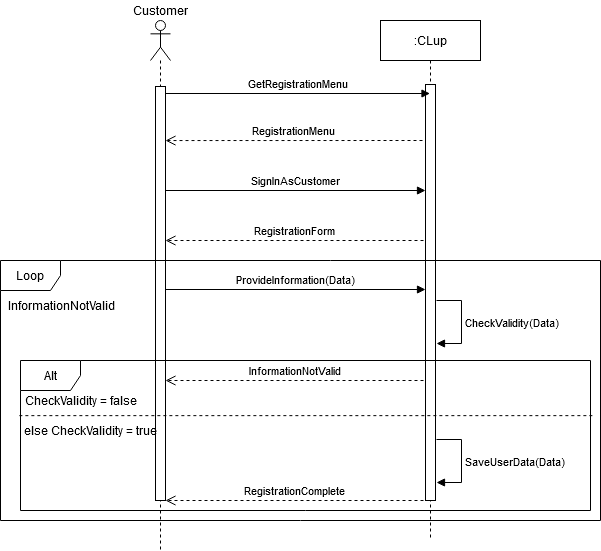
\includegraphics[scale=0.5]{Images/UseCase1Diagram.png}
\end{flushleft}
\paragraph{Store owner registration}
\begin{flushleft}
	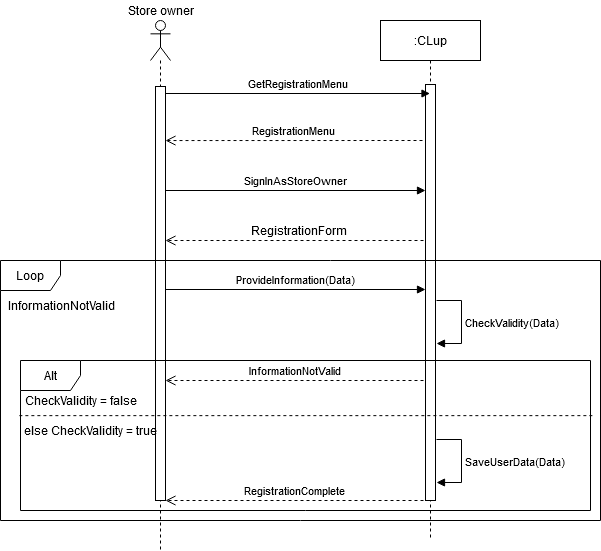
\includegraphics[scale=0.5]{Images/UseCase2Diagram.png}
\end{flushleft}
\newpage
\paragraph{User logs in}
\begin{flushleft}
	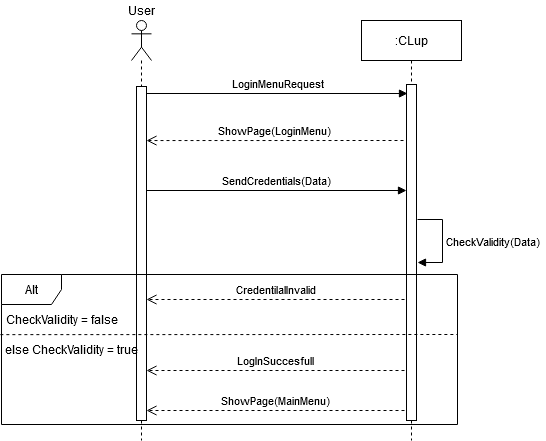
\includegraphics[scale=0.5]{Images/UseCase3Diagram.png}
\end{flushleft}
\paragraph{Customer queuing up remotely}
\begin{flushleft}
	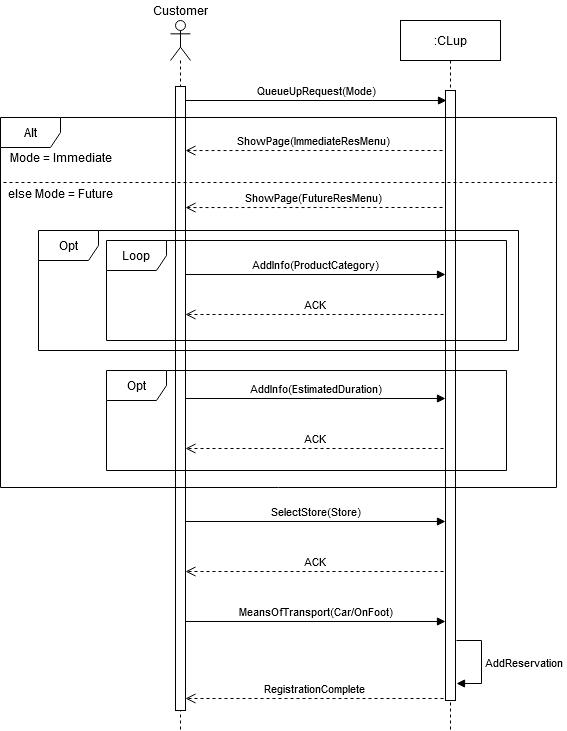
\includegraphics[scale=0.5]{Images/UseCase4Diagram.png}
\end{flushleft}
\newpage
\paragraph{Customer queuing up on premise}
\begin{flushleft}
	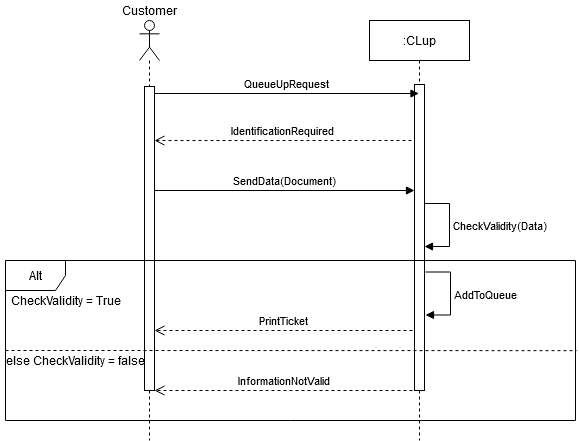
\includegraphics[scale=0.5]{Images/UseCase5Diagram.png}
\end{flushleft}
\paragraph{Customer entering and exiting store}
\begin{flushleft}
	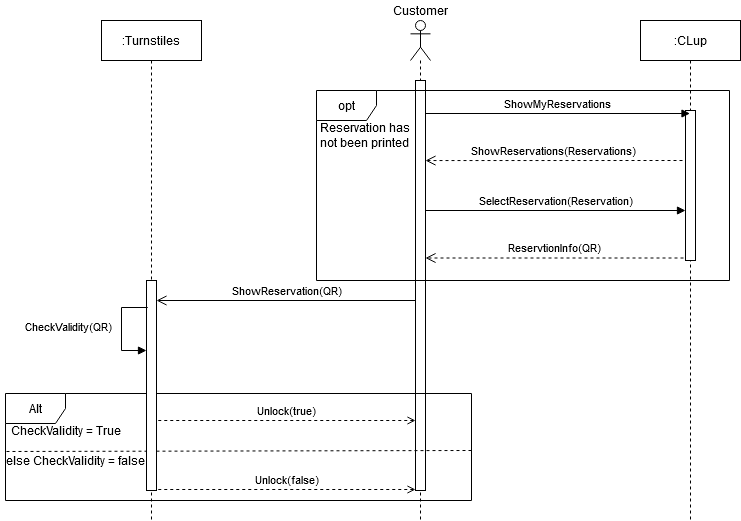
\includegraphics[scale=0.5]{Images/UseCase6-7Diagram.png}
\end{flushleft}
\newpage
\paragraph{Store owner registering a store}
\begin{flushleft}
	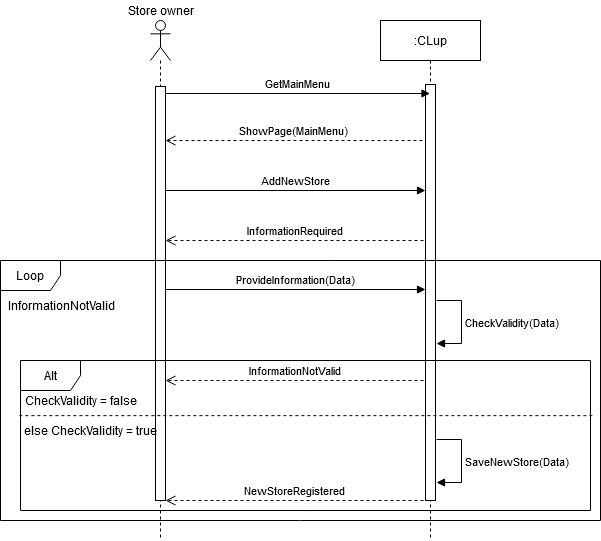
\includegraphics[scale=0.5]{Images/UseCase8Diagram.png}
\end{flushleft}
\paragraph{Store owner setting maximum occupation of a store or a department}
\begin{flushleft}
	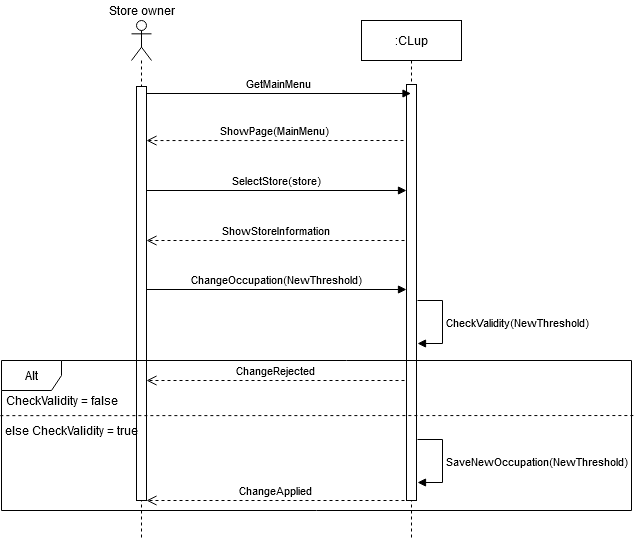
\includegraphics[scale=0.5]{Images/UseCase9Diagram.png}
\end{flushleft}
\newpage
\paragraph{Customer is alerted}
\begin{flushleft}
	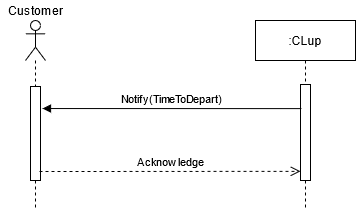
\includegraphics[scale=0.5]{Images/UseCase10Diagram.png}
\end{flushleft}

\subsection{Performance Requirements}
The system cannot guarantee that a customer can enter a store at a precise time unless it requires users to exit after a maximum time (which it doesn't).
The system guarantees that if
\begin{itemize}
	\item the customer uses a smartphone
	\item the customer never disconnects from the internet and GPS
	\item the customer specified the correct means of transport when creating the reservation
\end{itemize}
 he/she will be alerted when he needs to depart to reach a store (in order not to be late) with a delay of at most 10 seconds.
\subsection{Design Constraints}
\subsubsection{Standards compliance}
The code should follow the requirements contained in this document, and be thoroughly commented.
\subsubsection{Hardware limitations}
The software the customer uses requires either:
\begin{itemize}
	\item a smartphone to use the smart application
	\item a computer to use the web application and a home printer to print reservation
\end{itemize}
The software the store owner uses requires:
\begin{itemize}
	\item turnstiles activated by QR
	\item reservation printer activated by social security card
	\item monitor to alert on premise customers when it is their turn
\end{itemize}
\subsubsection{Any other constraint}
Customers cannot have more than five active reservation requests for different stores and more than two for the same store on the same day to avoid fake reservations.
\subsection{Software System Attributes}
\subsubsection{Reliability}
The system must have an appropriate infrastructure with a full backup system located in an separate office distant at least 100km (nuclear fallout radius). Adequate personnel will guarantee recovery time to substitute faulty hardware.
\subsubsection{Availability}
The system should be up for 99.9\% of the time (0.365 MTTR). Its temporary downtime does not cause emergency situations, but the system is an essential service: it should be possible to buy food every day. The system is fully automated. The users are alerted about system downtime with a delay of at most 10 minutes. The users are alerted that the system is up again with a delay of at most 10 minutes.
\subsubsection{Security}
The location of customers is sensitive information and therefore is never stored. Customers and store owners provide identifying information during registration: the databases containing such information must be protected against internal and external attacks. Communication between central system and users is encrypted.
\subsubsection{Maintainability}
The system is easy to maintain: its code is thoroughly commented and modular. Appropriate design patterns are exploited.
\subsubsection{Portability}
The smartphone application runs under Android and iOS. The web application runs under Android, iOS, Windows, MacOS.

%------------------------------------------------------------------------------------------------------------------------------------------------

\clearpage
{\color{Blue}{\section{Implementation, Integration and Test Plan}}}
\label{sect:alloy}
\subsection{Overview}
In this last section we provide all the necessary specifications about the plan for the implementation and the testing of the system. This phase is, of course, critical for the development of a reliable software system. It is important to observe that, while testing can show the presence of bugs in the code, passing the tests does not imply the absence of errors in the final application. Still, with our tests, we will try to find the majority of the bugs before the product hits the market (and also after, maintenance is important).

\subsection{Implementation Plan}
For all the implementation processes we have chosen a \textbf{bottom-up} approach; %TODO



The first element that we will implement is the DBMSServices component, which manages the model, i.e. the data, of our application, and so it is required by most of the components of the system.\\
After the data layer has been implemented we can proceed to the components that utilize it.
%bla bla bla queueManager blablabla

%------------------------------------------------------------------------------------------------------------------------------------------------

\clearpage
{\color{Blue}{\section{Effort Spent}}}
\label{sect:effort}
\subsection{Simone Abelli}
\begin{tabular} { | m{5cm} | m{1cm} | }
	\hline
	Introduction & 3.5\\
	\hline
	UML class diagram & 4\\
	\hline
	Product perspective & 3\\
	\hline
	State charts, External interface requirements & 4.5\\
	\hline
	User interfaces & 4.5\\
	\hline
	Requirements & 6.5\\
	\hline
	Sequence diagrams & 3.5\\
	\hline
	Scenarios & 0.5\\
	\hline
	Alloy & 7\\
	\hline
\end{tabular}

\subsection{Stefano Azzone}
\begin{tabular} { | m{5cm} | m{1cm} | }
	\hline
	Introduction & 3\\
	\hline
	UML class diagram & 3\\
	\hline
	Product perspective & 3\\
	\hline
	Product functions, user characteristics, domain assumptions & 2.5\\
	\hline
	State charts, External interface requirements & 3\\
	\hline
	Use cases & 3.5\\
	\hline
	Alloy & 11.5\\
	\hline
	Requirements & 6.5\\
	\hline
	Performance Requirements, Design constraints, Software system attributes, first two scenarios & 1\\
	\hline
\end{tabular}


%------------------------------------------------------------------------------------------------------------------------------------------------
\clearpage
\addcontentsline{toc}{section}{References}
\bibliographystyle{plain}
\bibliography{main}
\begin{itemize}
	\item \textbf{drawio.org} was used to draw diagrams
	\item \textbf{alloy.mit.edu} was the reference for alloy model
	\item \textbf{uml-diagrams.org} was the reference for uml diagrams
\end{itemize}
%------------------------------------------------------------------------------------------------------------------------------------------------




\end{document}
